\documentclass[11pt]{article}
% Adapted from an original template by Hlyni Arnórssyni,
% Reykjavik University, Iceland

% ------------------------------ PAGE SETTINGS ------------------------------
\usepackage{geometry}

\geometry{
    paper=a4paper,
    top=2.5cm,
    bottom=2.5cm,
    left=2.5cm,
    right=2.4cm,
    headheight=0.75cm,
    footskip=1.5cm,
    headsep=0.75cm
}

% ------------------------------ BASIC PACKAGES ------------------------------
\usepackage{blindtext}

% Character encoding
\usepackage[T1]{fontenc}
\usepackage[utf8]{inputenc}

% Mathematics
\usepackage{amsmath, amsfonts, amsthm, amssymb}
\usepackage{braket, nicefrac}

% SI units
\usepackage{siunitx}

% Lists / columns
\usepackage{enumitem, multicol}

% ------------------------------ FIGURES ------------------------------
\usepackage{graphicx}
\usepackage{float}
\usepackage{keystroke}
\usepackage{pgfplots}
\usepgfplotslibrary{units}
\pgfplotsset{compat=1.16}

% Search these locations automatically for figures
\graphicspath{{fig/}{graphics/}{Graphics/}{./}}

% ------------------------------ TABLES ------------------------------
\usepackage{tabularx}
\usepackage{array}
\usepackage[table]{xcolor}

% ------------------------------ TYPOGRAPHY ------------------------------
\usepackage{caption}
\usepackage{titlesec}
\usepackage{microtype}
\usepackage{csquotes}

% ------------------------------ COLORS ------------------------------
\definecolor{GWBlue}{HTML}{1E4E79}

% ------------------------------ SECTION STYLING ------------------------------
\titleformat{\section}
  {\Large\bfseries\color{GWBlue}}
  {\thesection.}
  {0.40em}
  {}

\titlespacing*{\section}
  {0pt}
  {0.70em}
  {0.28em}

% ------------------------------ CAPTION STYLING ------------------------------
\captionsetup{
    font=small,
    labelfont=bf,
    textfont=it,
    labelsep=period,
    skip=4pt
}

% ------------------------------ PARAGRAPH SPACING ------------------------------
\setlength{\parindent}{0pt}
\setlength{\parskip}{0.30em}

% ------------------------------ BIBLIOGRAPHY ------------------------------
\usepackage[
    backend=biber,
    style=authoryear,
    sorting=none,
    giveninits=true,
    maxbibnames=99,
    dashed=false
]{biblatex}

\addbibresource{references.bib}

\DeclareNameAlias{sortname}{family-given}
\DeclareNameAlias{default}{family-given}
\DeclareFieldFormat[article]{title}{#1}
\DeclareFieldFormat[misc]{title}{#1}
\renewbibmacro{in:}{}

\AtEveryBibitem{%
    \clearfield{doi}%
    \clearfield{urldate}%
}

\AtBeginBibliography{\small}
\setlength{\bibitemsep}{0.35em}

% ------------------------------ HYPERLINKS ------------------------------
\usepackage{hyperref}

\hypersetup{
    colorlinks=true,
    linkcolor=GWBlue,
    citecolor=GWBlue,
    urlcolor=GWBlue
}
\newcolumntype{C}[1]{>{\centering\arraybackslash}p{#1}}
\newcommand{\tbd}{\textbf{[TBD]}}
\setlength{\emergencystretch}{3em}
\graphicspath{{fig/}{fig/hard_example_mining/curriculum_comparison/}{fig/targeted_augmentation/augmentation_comparison/}{fig/som_reanalysis/}}
\usetikzlibrary{positioning,arrows.meta}
\begin{document}

\begin{titlepage}
\centering
\thispagestyle{empty}
\vspace*{0.15in}

\includegraphics[width=0.5\textwidth]{gwu_logo.pdf}
\vspace{0.28in}

{\large\bfseries Data Science Program\par}
{\large\bfseries Department of Data Science\par}
{\large DATS 6501 - Capstone Project - Fall 2026\par}
\vspace{0.38in}
{\Large\bfseries Post-Training Analysis \& Novelty Detection Using\par}
\vspace{0.08in}
{\Large\bfseries Neural Network Self-Organizing Maps (NNSOM)\par}
\vspace{0.34in}
{\large\bfseries PHASE 4 REPORT\par}
\vspace{0.22in}
{\large\bfseries Guided Retraining\par}
\vspace{0.36in}
{\large\bfseries Capstone - Group 5\par}
\vspace{0.08in}
{\large\bfseries Fyrooz Anika Khan\par}
{\large\bfseries Nazish Atta\par}
\vspace{0.30in}
{\large The George Washington University\par}
{\large Washington, DC\par}
\vspace{0.30in}
{\large\itshape Supervised by\par}
{\large\itshape Dr. Amir Jafari\par}
{\large\itshape Associate Professor of Data Science\par}
\vspace*{\fill}
\end{titlepage}

\section{Summary}

Phase 4 asks one question: \emph{can the SOM help us train a better CNN?} The SOM is a map that shows where the CNN makes its mistakes. We used it to pick the ``hard'' training images and then retrained the CNN (LeNet-5, on MNIST digits) in two ways: \textbf{curriculum learning} (the hard images are let in slowly) and \textbf{targeted augmentation} (we add slightly changed copies of the hard images). Every idea was compared with a fair control that uses the same number of images, repeated 5 times, and checked once on the test images. Last, we trained new SOMs on the retrained CNNs to see whether the map itself changed.

\begin{itemize}[leftmargin=1.4em, itemsep=1pt]
  \item \textbf{Targeted augmentation helped.} On the SOM's error regions (the ``hotspots''), mistakes fell from 11.4\% to 7.8\%. The rest of the images did not get worse.
  \item \textbf{Curriculum learning did not help.} It made the CNN slightly worse (98.66\% and 98.69\% correct, against 99.11\% for normal training).
  \item \textbf{The SOM is not the only way to pick hard images.} Picking the images the CNN is least sure about worked about as well, and the new SOMs after that augmentation cannot be told apart from those after SOM-guided augmentation. The SOM's real value is that it shows \emph{where} the errors are.
  \item \textbf{The new SOMs have smaller weak regions, but are not cleaner.} After augmentation the hotspots of a new SOM hold fewer mistakes than after normal training (17.5\% against 22.9\% on validation images). The neurons did not become purer, and against random copies the hotspot difference is not clear (Section~\ref{sec:reanalysis}).
  \item \textbf{The SOM still detects novel images after retraining.} Every retrained network's SOM separates SVHN from MNIST (AUROC 0.965 to 0.993). Whether SOM-guided retraining changes this could not be decided with 5 seeds (Section~\ref{sec:novelty_after}).
\end{itemize}

\subsection*{Where each item of the plan is covered}

{\small
\renewcommand{\arraystretch}{1.12}
\begin{tabularx}{\textwidth}{|>{\raggedright\arraybackslash}p{0.50\textwidth}|X|}
\hline
\textbf{What Phase 4 asks for} & \textbf{Where} \\ \hline
Hard-example pool and curriculum against standard training & Section~\ref{sec:method}, Tables~\ref{tab:arms}--\ref{tab:criteria}, Figures~\ref{fig:cf_cur} and~\ref{fig:curves} \\ \hline
Targeted augmentation and its effect on the rest of the data & Tables~\ref{tab:arms}--\ref{tab:criteria}, Figures~\ref{fig:cf_aug} and~\ref{fig:curves}, Appendix \\ \hline
Re-extract features, re-train the SOM, compare old and new maps & Section~\ref{sec:reanalysis}, Table~\ref{tab:reanalysis}, Figures~\ref{fig:reanalysis_measures}--\ref{fig:reanalysis_purity} \\ \hline
Feedback loop: SOM analysis $\rightarrow$ retraining $\rightarrow$ new SOM structure & Figure~\ref{fig:loop}, Section~\ref{sec:meaning} \\ \hline
Table: baseline accuracy, post-retraining accuracy & Table~\ref{tab:arms} \\ \hline
Table: novelty detection AUROC after retraining & Section~\ref{sec:novelty_after}, Table~\ref{tab:novelty_after} \\ \hline
Monitor forgetting of easy examples & Section~\ref{sec:meaning} (last item), Figure~\ref{fig:curves} \\ \hline
Before/after comparison and learning curves & Figures~\ref{fig:cf_aug}--\ref{fig:curves} \\ \hline
\end{tabularx}}

\section{Key terms in plain words}

\renewcommand{\arraystretch}{1.12}
{\small
\begin{tabularx}{\textwidth}{|>{\raggedright\arraybackslash}p{0.22\textwidth}|X|}
\hline
\textbf{Term} & \textbf{What it means} \\ \hline
CNN, LeNet-5 & The neural network that looks at a picture of a digit and says which digit it is. \\ \hline
SOM & A ``map'' that places similar images close together. We train it on what the CNN has learned, so we can see where the CNN gets confused. \\ \hline
Neuron, purity & A neuron is one cell of the map. Its purity is how many of its images show the same digit; low purity means a mixed, confusing cell. \\ \hline
Hotspot & A map cell where the CNN makes many mistakes (11 cells in our map). \\ \hline
Hard image, pool & A training image that sits in a hotspot, in a mixed cell, or far from its cell. All hard images together are the \emph{pool} (4{,}217 images). \\ \hline
Curriculum learning & Teach like school: start with easy images and let the hard ones in step by step. \\ \hline
Augmentation & Adding copies of an image that are slightly changed (turned, shifted, zoomed, sheared) so the CNN sees more variety. \\ \hline
Control & A fair comparison that uses the same number of added images but picks them differently: \emph{random} (by chance) or \emph{msp} (the images the CNN is least sure about). \\ \hline
Max-softmax (MSP) & The CNN's confidence in its answer. Low confidence means ``not sure''. \\ \hline
Seed & A number that fixes the randomness of one training run. We repeat every experiment with 5 seeds so one lucky run does not fool us. \\ \hline
Validation / test images & Validation images are used while building and checking the method. Test images are kept untouched and used once at the end, like an exam. \\ \hline
Error, accuracy & Error is the share of images the CNN gets wrong; accuracy is the share it gets right. \\ \hline
Confusion matrix (CF1, CF2) & A table of true digit against predicted digit; the diagonal is correct answers, everything else is mistakes. CF1 is before retraining (normal training), CF2 is after. \\ \hline
95\% interval & The range in which the true difference very likely lies. If it does not include 0, the difference is probably real and not luck. \\ \hline
Paired difference & Two methods compared seed by seed (the same seed for both), so that the comparison is fair. \\ \hline
Macro-F1 guard & A safety check that the CNN did not get worse on some digits while improving on others. \\ \hline
Forgetting & The CNN becoming worse on images it already handled well after being retrained. \\ \hline
Weighted purity & The share of images that show the main digit of their neuron. Higher means cleaner class regions. \\ \hline
Class scatter index & How many separate patches of the map one digit occupies on average. 1 means every digit has one connected region. \\ \hline
Topographic error & The share of images whose two closest neurons are not neighbours on the map. Lower means a better ordered map. \\ \hline
CKA & A score from 0 to 1 for how similar the embeddings of two networks are; 1 means the same. \\ \hline
\end{tabularx}}

\section{Method}\label{sec:method}

The loop is: SOM analysis $\rightarrow$ targeted retraining $\rightarrow$ re-analysis (Figure~\ref{fig:loop}). The retraining algorithm is fixed in advance and is the same for every arm.

\begin{figure}[H]
\centering
\begin{tikzpicture}[
  font=\footnotesize, node distance=9mm,
  box/.style={draw=GWBlue, rounded corners=2pt, align=center, minimum height=13mm, minimum width=42mm, fill=GWBlue!6, line width=0.6pt},
  arr/.style={-{Stealth[length=2mm]}, line width=0.7pt, draw=GWBlue}]
\node[box] (a) {\textbf{1. SOM analysis}\\ 11 hotspot neurons,\\ 4{,}217 hard training images};
\node[box, right=of a] (b) {\textbf{2. Targeted retraining}\\ curriculum or\\ augmented copies};
\node[box, right=of b] (c) {\textbf{3. New SOMs}\\ trained on the retrained\\ CNNs, 15 maps};
\draw[arr] (a)--(b); \draw[arr] (b)--(c);
\draw[arr, dashed] (c.south) -- ++(0,-6mm) -| (a.south);
\end{tikzpicture}
\caption{The feedback loop of Phase 4. The dashed arrow marks the next round, which this report does not run.}
\label{fig:loop}
\end{figure}

\begin{enumerate}[leftmargin=1.6em, itemsep=1pt]
  \item \textbf{Select hard images (training images only, true labels).} A training image is in the \emph{SOM pool} if its neuron is one of the 11 error hotspots, or its neuron's purity is below 0.95, or its distance to its neuron is above the 95th percentile. This gives 4{,}217 of 49{,}000 images (8.6\%). A smaller \emph{hotspot pool} (685 images) uses the first rule only.
  \item \textbf{Build controls of the same size.} \emph{random}: random images with the same digit mix, redrawn for each seed. \emph{msp}: the images with the lowest max-softmax confidence. \emph{standard}: nothing added.
  \item \textbf{Retrain from scratch, once per arm.} LeNet-5 \parencite{lecun1998gradient} with the Phase 1 recipe (Adam \parencite{kingma2015adam}, 20 epochs), seeds 1 to 5, the same seeds for all arms.
  \begin{itemize}[leftmargin=1.2em, itemsep=0pt]
    \item \emph{Curriculum:} all easy images plus 10\% of the hard pool, with 10\% more every 5 epochs (easiest first), so the last epochs use 40\% of the pool.
    \item \emph{Augmentation:} all original images plus 3 altered copies of every pool image (rotation up to 10$^\circ$, shift up to 1 pixel, zoom 0.9 to 1.1, shear up to 8$^\circ$). Two \emph{paced} arms add the same copies gradually, as in the curriculum.
  \end{itemize}
  \item \textbf{Evaluate once on the test split (10{,}500 images).} CF1 is the confusion matrix of the \texttt{standard} arm, CF2 that of a retrained arm. Differences between arms are paired bootstrap intervals over the test images (2{,}000 resamples), computed on the mean of the 5 seeds.
\end{enumerate}

\begin{table}[H]
\centering
\renewcommand{\arraystretch}{1.1}
\small
\begin{tabular}{|l|C{0.11\textwidth}|C{0.13\textwidth}|C{0.17\textwidth}|}
\hline
\textbf{Pool (training images)} & \textbf{Images} & \textbf{Share of 49,000} & \textbf{Training errors inside} \\ \hline
On a hotspot neuron (hotspot pool) & 685 & 1.4\% & 7 \\ \hline
In a neuron with purity $<0.95$ & 2,147 & 4.4\% & 16 \\ \hline
Distance to neuron above the 95th percentile & 2,450 & 5.0\% & 4 \\ \hline
\textbf{SOM pool} (any of the three) & \textbf{4,217} & \textbf{8.6\%} & \textbf{18} \\ \hline
msp pool (same size) & 4,217 & 8.6\% & 28 \\ \hline
In both the SOM and the msp pool & 1,965 & 4.0\% & 18 \\ \hline
\end{tabular}
\caption{The hard-image pools. The Phase 1 network makes only 29 mistakes on the training images; 18 of them are in the SOM pool and 28 in the msp pool. By digit, the SOM pool is largest for digit 2 (984 images) and smallest for digit 1 (146). Each augmentation arm adds 3 altered copies of every pool image, 12,651 images. Source: \texttt{tables/hard\_example\_mining/hard\_example\_pools/}.}
\label{tab:pools}
\end{table}

\textbf{Success criteria} (written down before the test split was used): C1, curriculum\_som has lower overall error than standard; C2, curriculum\_som has lower hotspot error than curriculum\_random; A1, augmented\_som has lower hotspot error than augmented\_random; A2, augmented\_som has lower hotspot error than standard; A3, augmented\_som does not raise the error outside the hotspots by more than 0.2 points. C1, C2, A1 and A2 also need an interval that excludes 0 and a macro-F1 that does not fall by more than 0.0016.

\subsection*{Re-analysis with new SOMs}

The last step of the loop retrains nothing. For the \texttt{standard}, \texttt{augmented\_som} and \texttt{augmented\_random} arms and each of the 5 CNN seeds, we took the 84-dimensional embeddings of the training and validation images, trained a new 15$\times$15 SOM with the Phase 2 recipe (neighbourhood 11, 250 epochs, seed 42), and measured it on the validation split only; the test split was not read. That gives 15 new SOMs, plus the Phase 2 map as a read-only reference. The measures are weighted purity, the share of low-purity neurons ($<0.95$), a class scatter index, topographic error, the error rate on the 11 worst neurons (hotspots, picked by the lower Wilson bound of their error rate), the share of all errors that fall on those neurons, overall error, and linear CKA \parencite{kornblith2019cka} between networks. The first four follow the SOM quality measures surveyed by \textcite{forest2020somsurvey}; the class scatter index is our own implementation of their verbal description. Differences between arms are taken per seed, since the arms share seeds \parencite{bouthillier2021variance}, then averaged, with a 95\% $t$-interval over the 5 differences. The five statements below (R1 to R5) and the tolerance of 1.0 percentage point in R5 were written down before the run.

\begin{itemize}[leftmargin=1.4em, itemsep=1pt]
  \item R1: purity is higher for \texttt{augmented\_som} than for \texttt{standard} (interval above 0).
  \item R2: hotspot error rate is lower for \texttt{augmented\_som} than for \texttt{standard} (interval below 0).
  \item R3: purity is higher for \texttt{augmented\_som} than for \texttt{augmented\_random}.
  \item R4: hotspot error rate is lower for \texttt{augmented\_som} than for \texttt{augmented\_random}.
  \item R5: topographic error of \texttt{augmented\_som} is not more than 1.0 point above \texttt{standard} (upper end of the interval at most 1.0).
\end{itemize}

\section{Results of the retraining}

Table~\ref{tab:arms} gives baseline and post-retraining accuracy; Table~\ref{tab:criteria} gives the verdicts. Figures~\ref{fig:cf_aug} and~\ref{fig:cf_cur} show CF1 and CF2 (the other arms are in the Appendix), and Figure~\ref{fig:curves} the learning curves.

\begin{table}[H]
\centering
\renewcommand{\arraystretch}{1.1}
\small
\begin{tabular}{|l|C{0.20\textwidth}|C{0.20\textwidth}|C{0.20\textwidth}|}
\hline
\textbf{Arm} & \textbf{Test accuracy (\%)} & \textbf{Hotspot error (\%)} & \textbf{Non-hotspot error (\%)} \\ \hline
\textbf{standard} (baseline, CF1) & 99.11 (0.12) & 11.4 (2.6) & 0.74 (0.10) \\ \hline
\multicolumn{4}{|l|}{\textit{Curriculum}} \\ \hline
curriculum\_som & 98.66 (0.04) & 21.4 (2.9) & 1.05 (0.06) \\ \hline
curriculum\_random & 99.07 (0.05) & 12.2 (2.3) & 0.77 (0.03) \\ \hline
curriculum\_msp & 98.69 (0.08) & 22.6 (3.3) & 1.01 (0.06) \\ \hline
\multicolumn{4}{|l|}{\textit{Targeted augmentation}} \\ \hline
augmented\_som & 99.21 (0.07) & 7.8 (2.6) & 0.69 (0.05) \\ \hline
augmented\_random & 99.18 (0.05) & 10.3 (2.4) & 0.68 (0.05) \\ \hline
augmented\_msp & 99.25 (0.06) & 8.5 (1.2) & 0.64 (0.06) \\ \hline
augmented\_hotspot & 99.14 (0.08) & 9.5 (2.9) & 0.74 (0.05) \\ \hline
augmented\_random\_hotspot & 99.12 (0.09) & 11.6 (2.9) & 0.73 (0.06) \\ \hline
augmented\_som\_paced & 99.12 (0.09) & 11.2 (3.6) & 0.73 (0.06) \\ \hline
augmented\_random\_paced & 99.11 (0.04) & 11.5 (2.1) & 0.74 (0.06) \\ \hline
\end{tabular}
\caption{Test results, mean (standard deviation) over 5 seeds. Hotspot error is measured on the 146 test images that fall on hotspot neurons, non-hotspot error on the other 10,354. Both experiments use the same \texttt{standard} arm.}
\label{tab:arms}
\end{table}


\begin{table}[H]
\centering
\renewcommand{\arraystretch}{1.12}
\small
{\setlength{\tabcolsep}{3pt}\begin{tabular}{|C{0.06\textwidth}|>{\raggedright\arraybackslash}p{0.38\textwidth}|C{0.22\textwidth}|C{0.14\textwidth}|C{0.10\textwidth}|}
\hline
\textbf{ID} & \textbf{Comparison (error on)} & \textbf{Difference in points [95\% CI]} & \textbf{Macro-F1 guard} & \textbf{Verdict} \\ \hline
C1 & curriculum\_som $-$ standard (all test images) & +0.45 [+0.33, +0.57] & $-$0.0044 (fails) & \textbf{not met} \\ \hline
C2 & curriculum\_som $-$ curriculum\_random (hotspots) & +9.18 [+5.48, +13.02] & $-$0.0040 (fails) & \textbf{not met} \\ \hline
A1 & augmented\_som $-$ augmented\_random (hotspots) & $-$2.47 [$-$4.52, $-$0.68] & +0.0003 (holds) & \textbf{met} \\ \hline
A2 & augmented\_som $-$ standard (hotspots) & $-$3.56 [$-$5.75, $-$1.37] & +0.0010 (holds) & \textbf{met} \\ \hline
A3 & augmented\_som $-$ standard (non-hotspot images; limit: upper end $\le 0.2$) & $-$0.05 [$-$0.13, +0.02] &  & \textbf{met} \\ \hline
\multicolumn{5}{|l|}{\textit{Also reported (not success criteria)}} \\ \hline
R1 & augmented\_som $-$ augmented\_msp (hotspots) & $-$0.68 [$-$2.88, +1.23] &  & \textbf{tie} \\ \hline
R2 & augmented\_som\_paced $-$ augmented\_som (hotspots) & +3.42 [+1.64, +5.34] &  & \textbf{worse} \\ \hline
R3 & augmented\_hotspot $-$ augmented\_random\_hotspot (hotspots) & $-$2.19 [$-$4.52, +0.14] &  & \textbf{tie} \\ \hline
\end{tabular}}
\caption{The success criteria, fixed before the test split was used. Negative differences mean fewer errors for the first arm; 1 test hotspot image is about 0.7 points. Intervals: paired bootstrap over test images, mean of 5 seeds. The macro-F1 guard is the first arm's macro-F1 minus the second arm's; it may not fall below $-0.0016$.}
\label{tab:criteria}
\end{table}


\textbf{Every arm against normal training.} The protocol also asks for every arm compared with \texttt{standard} (Table~\ref{tab:vs_standard}; not success criteria). All three full-pool augmentation arms lower the overall test error by a small amount whose interval excludes 0, including random copies ($-0.07$ points) and least-confident copies ($-0.14$ points), so part of the gain comes from adding altered copies of any images. Only \texttt{augmented\_som} also has a hotspot interval that excludes 0. The hotspot-pool and paced arms do not differ clearly from \texttt{standard}. The paced arms are worse than their unpaced twins on overall error (+0.07 points for random, +0.09 for SOM copies), and the two paced arms cannot be told apart on the hotspots ($-0.27$ points, $-2.47$ to $+1.92$). Random-order curriculum is not clearly worse than \texttt{standard}; the SOM and least-confident orders are.

\begin{table}[H]
\centering
\renewcommand{\arraystretch}{1.1}
\footnotesize
{\setlength{\tabcolsep}{4pt}\begin{tabular}{|l|C{0.22\textwidth}|C{0.22\textwidth}|C{0.22\textwidth}|}
\hline
\textbf{Arm $-$ standard} & \textbf{All test images} & \textbf{Hotspot images} & \textbf{Non-hotspot images} \\ \hline
augmented\_som & \textbf{$-$0.10 [$-$0.18, $-$0.02]} & \textbf{$-$3.56 [$-$5.75, $-$1.37]} & $-$0.05 [$-$0.13, +0.02] \\ \hline
augmented\_random & \textbf{$-$0.07 [$-$0.13, $-$0.01]} & $-$1.10 [$-$3.42, +1.37] & $-$0.06 [$-$0.11, +0.00] \\ \hline
augmented\_msp & \textbf{$-$0.14 [$-$0.23, $-$0.04]} & $-$2.88 [$-$6.16, +0.28] & \textbf{$-$0.10 [$-$0.18, $-$0.02]} \\ \hline
augmented\_hotspot & $-$0.03 [$-$0.10, +0.04] & $-$1.92 [$-$4.38, +0.68] & 0.00 [$-$0.06, +0.05] \\ \hline
augmented\_random\_hotspot & $-$0.01 [$-$0.07, +0.05] & +0.27 [$-$1.51, +2.19] & $-$0.01 [$-$0.07, +0.04] \\ \hline
augmented\_som\_paced & $-$0.01 [$-$0.08, +0.06] & $-$0.14 [$-$2.74, +2.33] & $-$0.01 [$-$0.07, +0.06] \\ \hline
augmented\_random\_paced & +0.00 [$-$0.06, +0.06] & +0.14 [$-$1.78, +2.05] & +0.00 [$-$0.05, +0.06] \\ \hline
curriculum\_som & \textbf{+0.45 [+0.33, +0.57]} & \textbf{+10.00 [+6.30, +13.70]} & \textbf{+0.31 [+0.20, +0.42]} \\ \hline
curriculum\_random & +0.04 [$-$0.02, +0.11] & +0.82 [$-$1.51, +3.15] & +0.03 [$-$0.03, +0.09] \\ \hline
curriculum\_msp & \textbf{+0.42 [+0.30, +0.54]} & \textbf{+11.23 [+7.12, +15.48]} & \textbf{+0.27 [+0.16, +0.38]} \\ \hline
\end{tabular}}
\caption{Every arm minus \texttt{standard}: difference in test error, percentage points, with the 95\% paired bootstrap interval over test images (mean of 5 seeds). Bold: the interval excludes 0. Also reported, not success criteria. Source: \texttt{test\_comparisons.csv} of the two comparison folders under \texttt{tables/}.}
\label{tab:vs_standard}
\end{table}

\textbf{Validation results.} The validation split was used before the test pass, for the checks only: the macro-F1 guard is twice the standard deviation of the \texttt{standard} row's macro-F1 ($2\times0.0008=0.0016$). Table~\ref{tab:validation} gives every arm on it, for completeness; no arm, threshold or setting was chosen from it. The ordering is the same as on the test split: \texttt{augmented\_som} and \texttt{augmented\_msp} have the lowest hotspot error, and the SOM and least-confident curricula the highest.

\begin{table}[H]
\centering
\renewcommand{\arraystretch}{1.1}
\footnotesize
\begin{tabular}{|l|C{0.18\textwidth}|C{0.18\textwidth}|C{0.18\textwidth}|}
\hline
\textbf{Arm} & \textbf{Validation error (\%)} & \textbf{Hotspot error (\%)} & \textbf{Macro-F1} \\ \hline
standard & 0.92 (0.08) & 16.4 (1.3) & 0.9908 (0.0008) \\ \hline
\multicolumn{4}{|l|}{\textit{Curriculum}} \\ \hline
curriculum\_som & 1.44 (0.04) & 24.7 (1.7) & 0.9855 (0.0004) \\ \hline
curriculum\_random & 0.96 (0.07) & 17.4 (1.0) & 0.9903 (0.0008) \\ \hline
curriculum\_msp & 1.51 (0.03) & 24.9 (1.2) & 0.9848 (0.0004) \\ \hline
\multicolumn{4}{|l|}{\textit{Targeted augmentation}} \\ \hline
augmented\_som & 0.75 (0.08) & 12.1 (1.1) & 0.9924 (0.0008) \\ \hline
augmented\_random & 0.86 (0.11) & 15.7 (2.2) & 0.9913 (0.0011) \\ \hline
augmented\_msp & 0.70 (0.05) & 12.5 (1.5) & 0.9930 (0.0006) \\ \hline
augmented\_hotspot & 0.82 (0.08) & 13.1 (0.9) & 0.9917 (0.0008) \\ \hline
augmented\_random\_hotspot & 0.91 (0.06) & 16.1 (1.8) & 0.9908 (0.0006) \\ \hline
augmented\_som\_paced & 0.87 (0.04) & 15.9 (1.2) & 0.9913 (0.0004) \\ \hline
augmented\_random\_paced & 0.91 (0.05) & 16.3 (2.1) & 0.9909 (0.0005) \\ \hline
\end{tabular}
\caption{Validation results, mean (standard deviation) over 5 seeds, on the 10,500 validation images; hotspot error is on the validation images that fall on the 11 hotspot neurons. Source: \texttt{tables/validation\_summary.csv} of the two comparison runs.}
\label{tab:validation}
\end{table}

\begin{figure}[H]
\centering
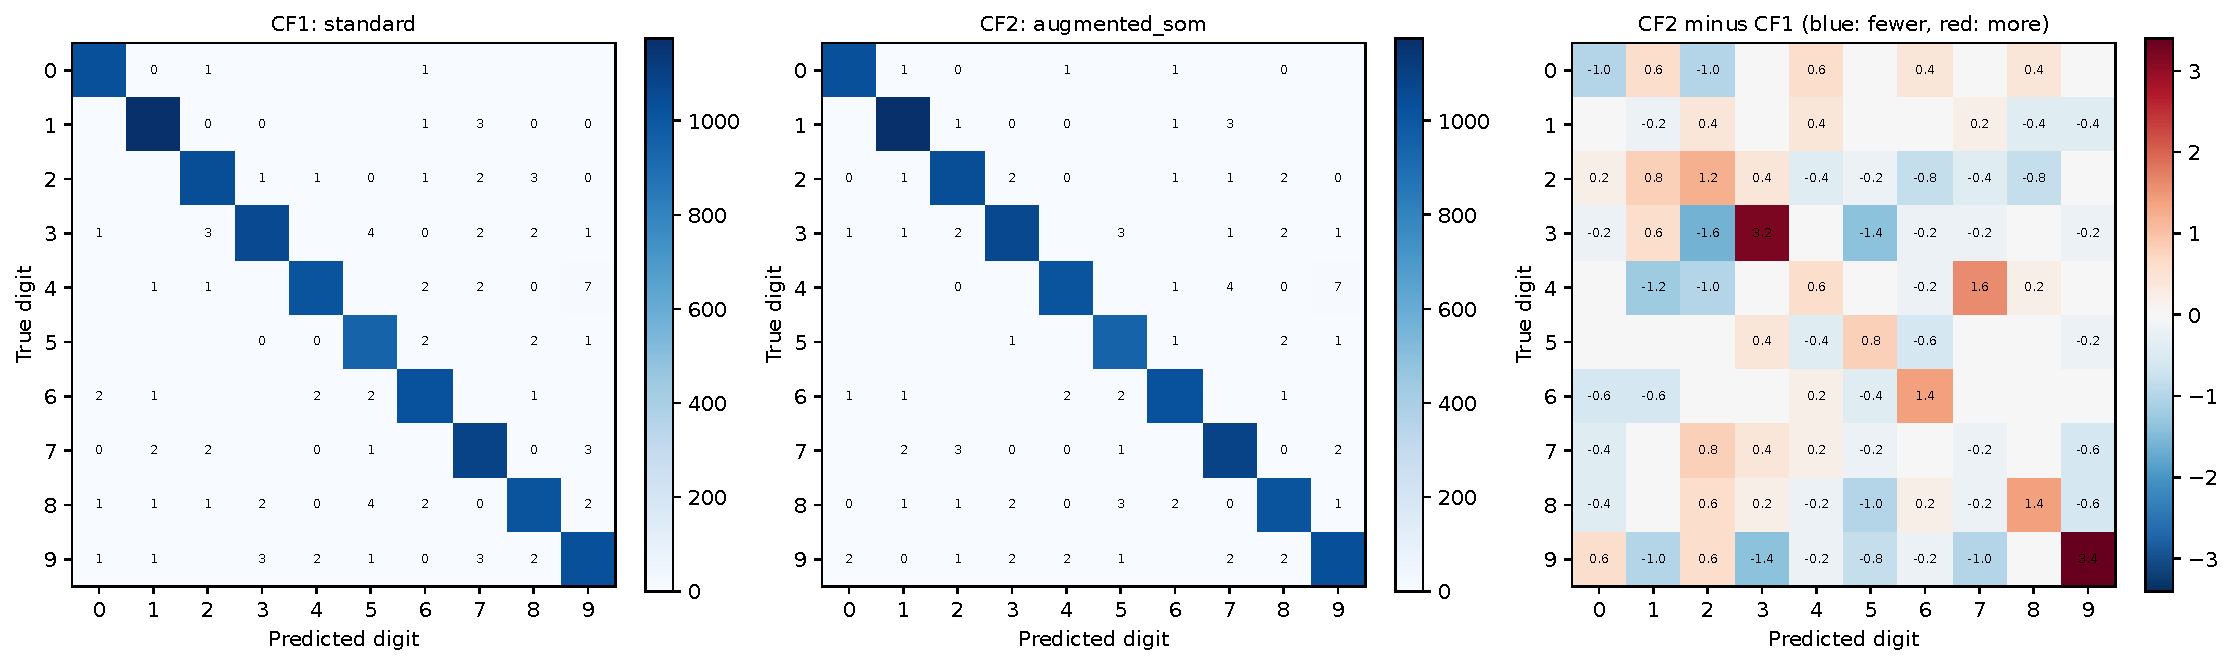
\includegraphics[width=\textwidth]{fig/targeted_augmentation/augmentation_comparison/confusion_standard_vs_augmented_som.pdf}
\caption{CF1 (standard) and CF2 (augmented\_som): mean test confusion matrices over 5 seeds, and their difference (blue: fewer cases, red: more).}
\label{fig:cf_aug}
\end{figure}

\begin{figure}[H]
\centering
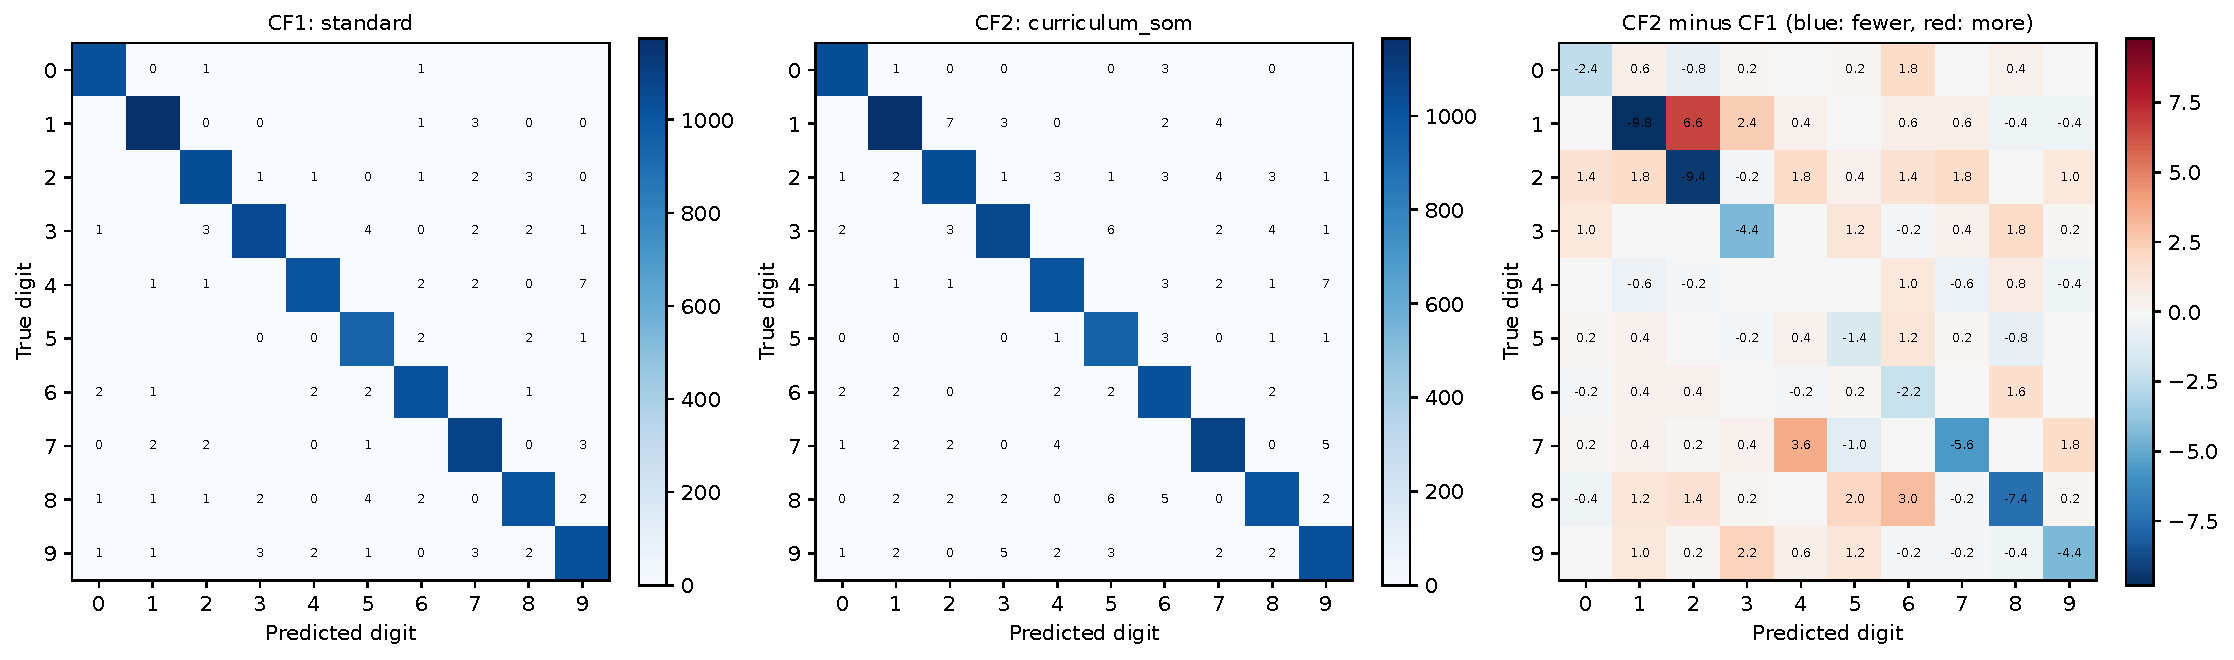
\includegraphics[width=\textwidth]{fig/hard_example_mining/curriculum_comparison/confusion_standard_vs_curriculum_som.pdf}
\caption{CF1 (standard) and CF2 (curriculum\_som), as in Figure~\ref{fig:cf_aug}.}
\label{fig:cf_cur}
\end{figure}

\begin{figure}[H]
\centering
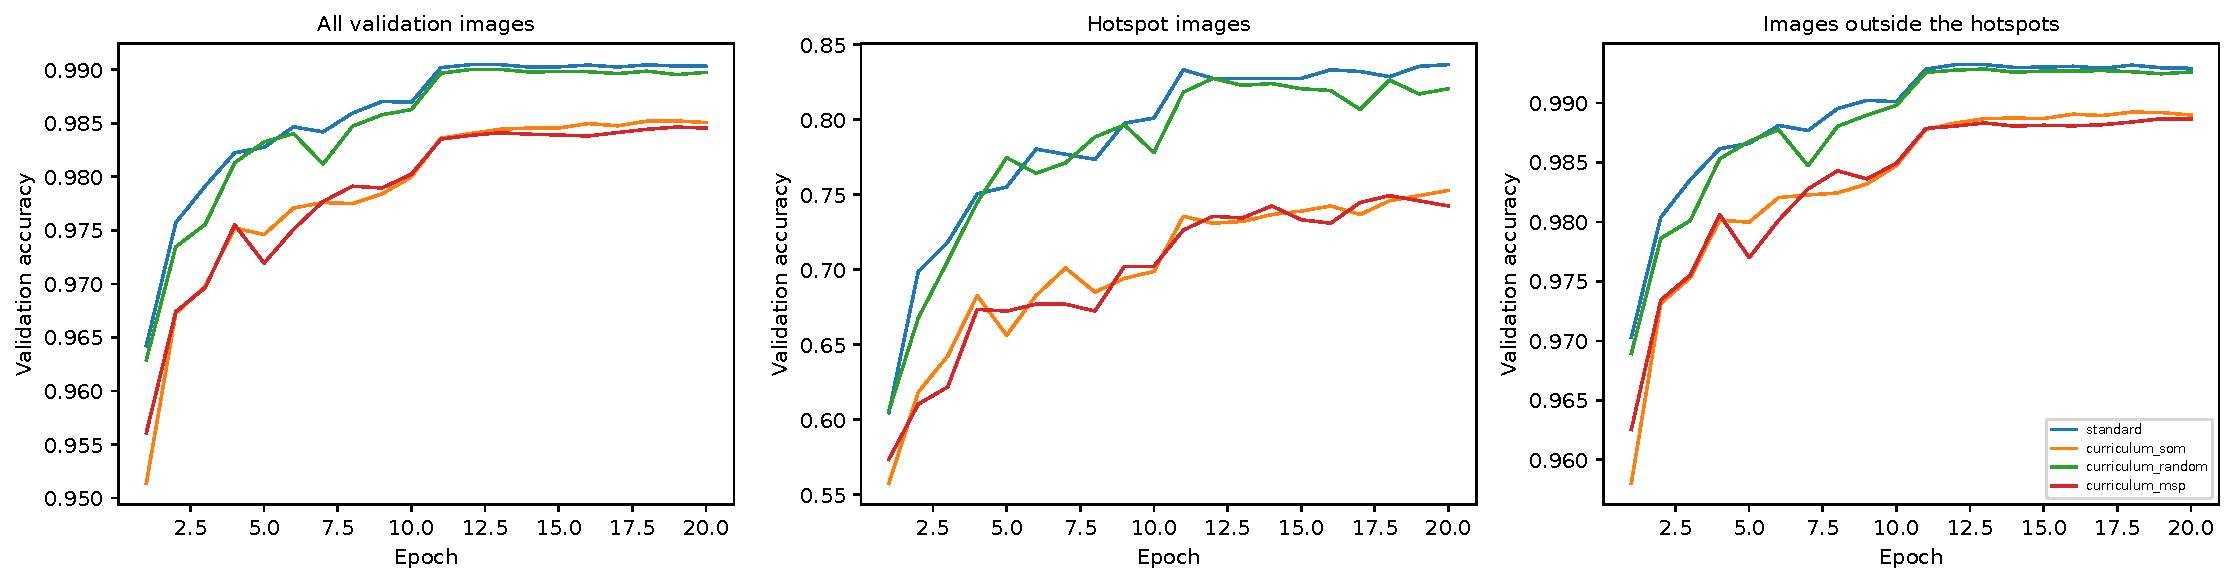
\includegraphics[width=\textwidth]{fig/hard_example_mining/curriculum_comparison/validation_accuracy_by_epoch.pdf}
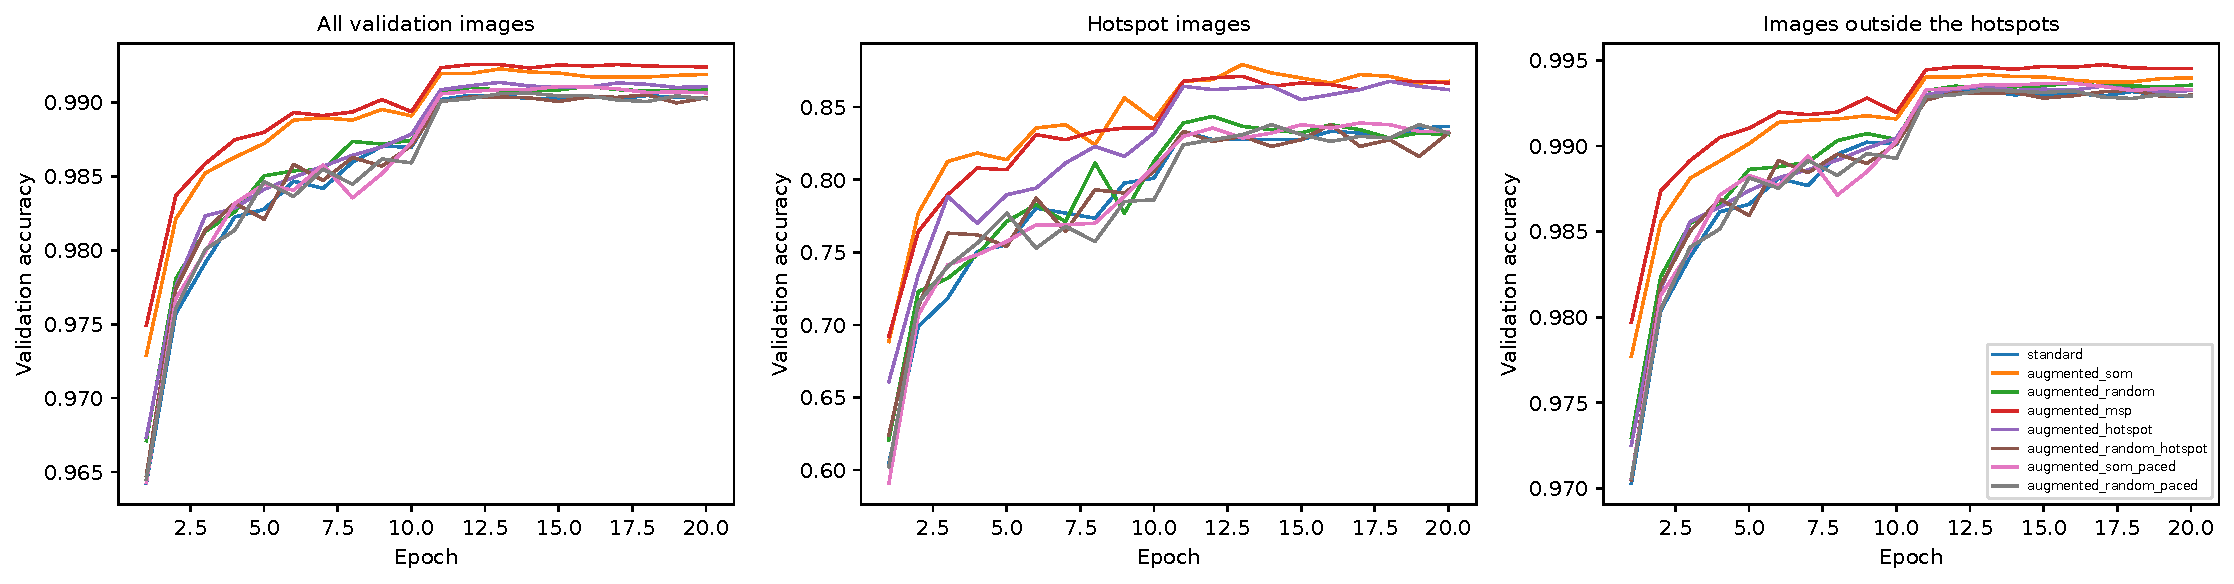
\includegraphics[width=\textwidth]{fig/targeted_augmentation/augmentation_comparison/validation_accuracy_by_epoch.pdf}
\caption{Validation accuracy per epoch (mean of 5 seeds) for the curriculum arms (top) and the augmentation arms (bottom): all images, hotspot images, and images outside the hotspots.}
\label{fig:curves}
\end{figure}

\section{Re-analysis: new SOMs after retraining}\label{sec:reanalysis}

Table~\ref{tab:reanalysis} gives all measures and Figures~\ref{fig:reanalysis_measures} and~\ref{fig:reanalysis_purity} show the spread over seeds and example maps. Two of the five statements hold (R2, R5) and three do not (R1, R3, R4).

\begin{table}[H]
\centering
\renewcommand{\arraystretch}{1.12}
\footnotesize
{\setlength{\tabcolsep}{3pt}\begin{tabular}{|>{\raggedright\arraybackslash}p{0.18\textwidth}|C{0.08\textwidth}|C{0.085\textwidth}|C{0.09\textwidth}|C{0.09\textwidth}|C{0.185\textwidth}|C{0.185\textwidth}|}
\hline
\textbf{Measure (validation)} & \textbf{Phase 2 map} & \textbf{standard} & \textbf{augm.\ som} & \textbf{augm.\ random} & \textbf{augm.\ som $-$ standard} & \textbf{augm.\ som $-$ augm.\ random} \\ \hline
Weighted purity (R1, R3) & 0.9819 & 0.9824 & 0.9824 & 0.9813 & +0.0001 [$-$0.0017, +0.0019] & +0.0012 [$-$0.0016, +0.0039] \\ \hline
Share of neurons with purity $<0.95$ & 0.0801 & 0.0718 & 0.0795 & 0.0758 & +0.0077 [$-$0.0045, +0.0199] & +0.0037 [$-$0.0114, +0.0188] \\ \hline
Class scatter index & 1.10 & 1.12 & 1.20 & 1.12 & +0.08 [$-$0.14, +0.30] & +0.08 [$-$0.12, +0.28] \\ \hline
Topographic error, \% (R5) & 6.18 & 7.04 & 6.76 & 6.66 & $-$0.29 [$-$1.11, +0.54] & +0.10 [$-$1.04, +1.25] \\ \hline
Hotspot error rate (R2, R4) & 0.1954 & 0.2292 & 0.1746 & 0.2061 & \textbf{$-$0.0545 [$-$0.1008, $-$0.0082]} & $-$0.0315 [$-$0.0705, +0.0075] \\ \hline
Share of errors in hotspots & 0.3696 & 0.3669 & 0.3833 & 0.3204 & +0.0163 [$-$0.0613, +0.0939] & \textbf{+0.0628 [+0.0359, +0.0897]} \\ \hline
Overall validation error & 0.0088 & 0.0092 & 0.0075 & 0.0086 & \textbf{$-$0.0017 [$-$0.0022, $-$0.0011]} & \textbf{$-$0.0011 [$-$0.0018, $-$0.0005]} \\ \hline
\end{tabular}}
\caption{SOM re-analysis on the validation split. Columns 2 to 5 are means over the 5 CNN seeds (the Phase 2 map is a single map). The last two columns are the paired difference per seed, averaged, with its 95\% $t$-interval (4 degrees of freedom); bold means the interval excludes 0. Linear CKA between the networks' embeddings: 0.931 within standard, 0.893 within augmented\_som, 0.917 within augmented\_random, 0.910 between arms.}
\label{tab:reanalysis}
\end{table}


\begin{itemize}[leftmargin=1.4em, itemsep=2pt]
  \item \textbf{R1, not met.} Weighted purity of \texttt{augmented\_som} is the same as \texttt{standard} ($+0.0001$, interval $-0.0017$ to $+0.0019$). The class boundaries in the map did not become measurably sharper.
  \item \textbf{R2, met.} Hotspot error rate is lower by 5.5 points ($-0.0545$, interval $-0.1008$ to $-0.0082$), and it was lower in all 5 seeds.
  \item \textbf{R3, not met.} Against the random-image control the purity difference is $+0.0012$ with an interval from $-0.0016$ to $+0.0039$.
  \item \textbf{R4, not met.} Against the random-image control the hotspot error rate is lower by 3.1 points, but the interval ($-0.0705$ to $+0.0075$) includes 0, so we cannot say the SOM-chosen images are better than random ones here.
  \item \textbf{R5, met.} Topographic error did not rise ($-0.29$ points, interval $-1.11$ to $+0.54$; the upper end is below the 1.0 tolerance), so the map stayed as well ordered as after plain training.
  \item \textbf{Also reported.} The low-purity share and the class scatter index show no clear change. The share of all errors that sit in hotspots is larger than for the random control by $+0.063$ (larger in 5 of 5 seeds), but not larger than for \texttt{standard}. Overall validation error is lower for \texttt{augmented\_som} than for both other arms (about 0.17 and 0.11 points). CKA between networks is 0.89 to 0.93 within an arm and 0.91 between arms, so the arms do not differ more from each other than seeds do within an arm, except that \texttt{augmented\_som} networks are somewhat less alike (0.893). The mean quantization error of the new maps is 1.021 (\texttt{standard}), 1.084 (\texttt{augmented\_som}) and 1.053 (\texttt{augmented\_random}), against 1.041 for the Phase 2 map; each map is trained on a different network's embeddings, so these values are not directly comparable. Every new map uses 223 to 225 of its 225 neurons, and its 11 hotspots hold on average 160, 178 and 142 validation images (Phase 2 map: 174).
  \item \textbf{Secondary run: the least-confident arm.} Added after these results were seen (addendum \texttt{MSP\_ARM\_ADDENDUM.md}, run \texttt{som\_reanalysis\_msp\_arm\_som\_15x15\_nb11\_ep250\_s42\_v2}). The new maps of \texttt{augmented\_msp} have a hotspot error rate of 0.193 against 0.229 for \texttt{standard} ($-0.036$, interval $-0.093$ to $+0.021$, S1 not met). \texttt{augmented\_som} is not clearly better than \texttt{augmented\_msp} on hotspot error ($-0.018$, $-0.076$ to $+0.039$, S2 not met) or purity ($-0.0006$, $-0.0029$ to $+0.0017$, S3 not met). With 5 seeds no difference between SOM and confidence guidance can be shown. The \texttt{standard} and \texttt{augmented\_som} cells reproduced the primary run exactly.
\end{itemize}

\begin{figure}[H]
\centering
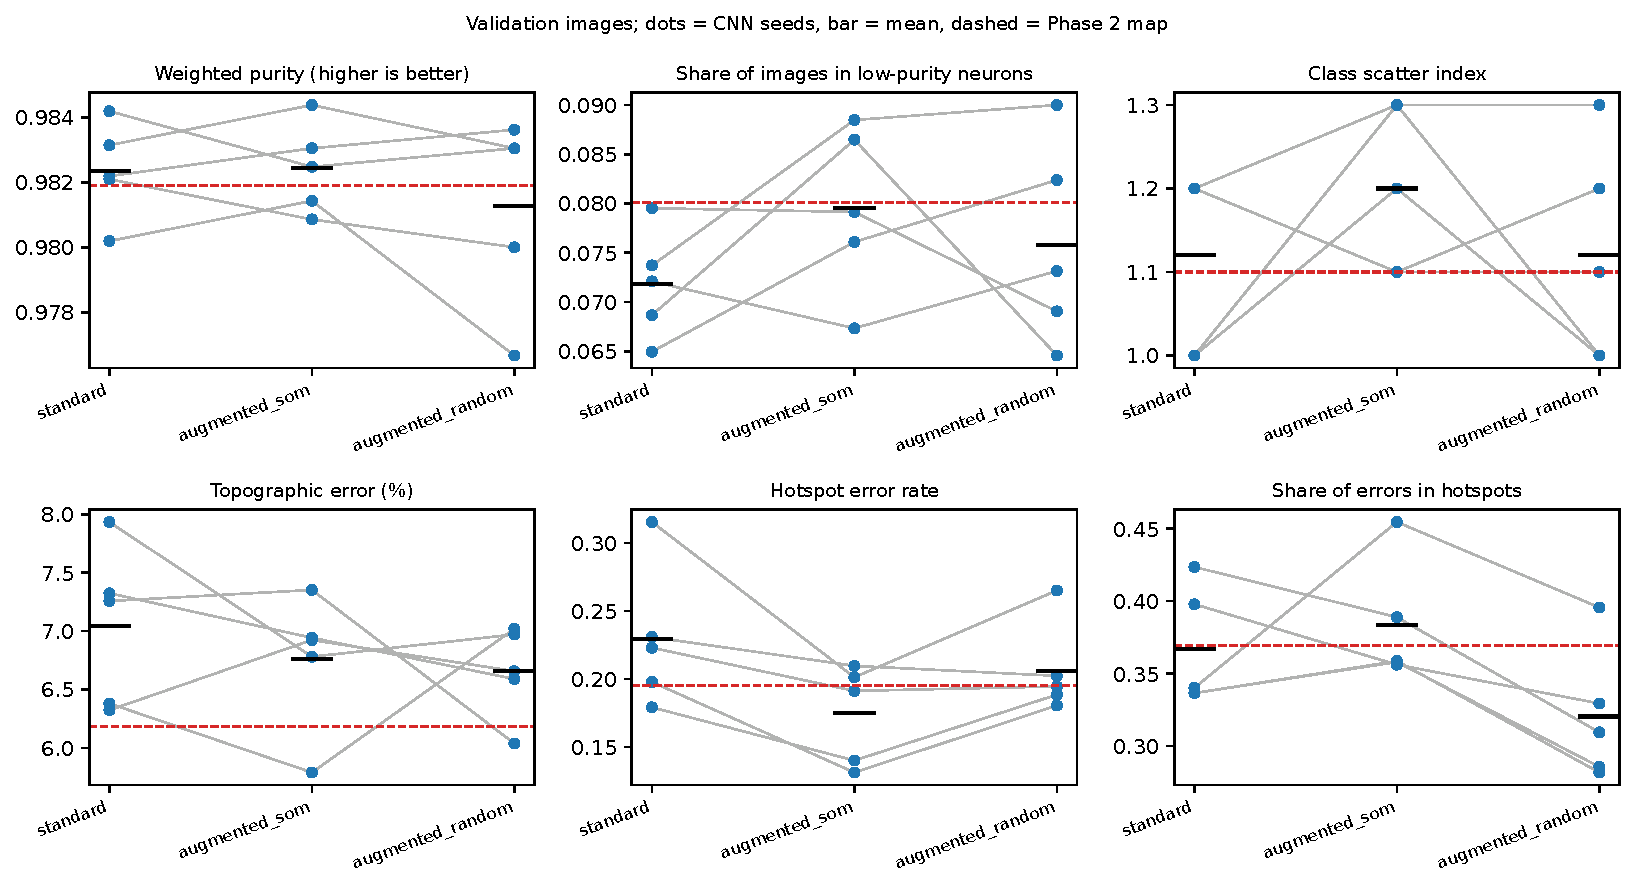
\includegraphics[width=\textwidth]{fig/som_reanalysis/map_measures_by_arm.pdf}
\caption{Map measures per arm on validation images. Each dot is one CNN seed (grey lines join the same seed), the black bar is the mean over seeds, and the red dashed line is the Phase 2 map.}
\label{fig:reanalysis_measures}
\end{figure}

\begin{figure}[H]
\centering
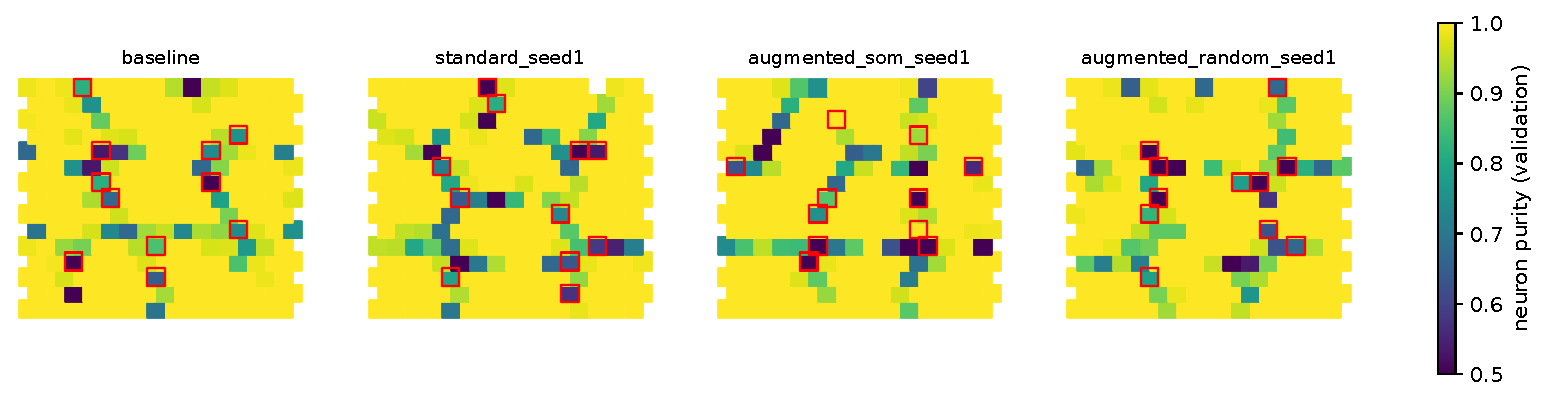
\includegraphics[width=\textwidth]{fig/som_reanalysis/purity_maps.pdf}
\caption{Neuron purity on validation images for the Phase 2 map and the three arms (seed 1). Red squares mark the hotspot neurons of each map. The hotspots are picked again for every map.}
\label{fig:reanalysis_purity}
\end{figure}

\textbf{How to read this.} Part of the hotspot drop comes from the network making fewer errors overall, not only on the weak regions. The hotspots are the worst neurons of each map, chosen again for every map, so the hotspot error rate of a new map is not measured on the same images as before. The retrained \texttt{standard} networks also have a higher hotspot error rate (0.229) than the Phase 2 map (0.195), so the Phase 2 map is not a fair baseline for the new ones; the comparison between arms is the one to use. With 5 seeds and one SOM seed the intervals are wide, and a clear result for one comparison next to an unclear one should not be over-read. All of this is on MNIST validation data.

\section{Errors fixed, and error per digit (exploratory)}\label{sec:breakdown}

Two questions from the reviews are answered here. Both were added on 2026-11-17, after the single test pass, from the test predictions saved by that pass: no network was retrained or re-run, and no criterion or threshold changed. They are descriptive, not success criteria.

\textbf{How many errors does retraining actually fix?} Percentages hide how few mistakes MNIST leaves, so Table~\ref{tab:errors_fixed} gives counts. Normal training makes about 93 errors on the 10{,}500 test images, 17 of them on the 146 hotspot images. Retraining moves many individual errors: \texttt{augmented\_som} fixes about 40 of \texttt{standard}'s errors per seed and makes about 30 new ones. On the hotspot images the net effect is consistent: \texttt{augmented\_som} has fewer hotspot errors than \texttt{standard} in all 5 seeds (1 to 8 fewer, about 5 on average), while \texttt{augmented\_random} and \texttt{augmented\_msp} each have at least one seed with more. Over all images the net gain is about 11 errors. The bootstrap interval over test images excludes 0 ($-0.10$ points, $-0.18$ to $-0.02$; Table~\ref{tab:vs_standard}), but the gain varies from $-12$ to $+31$ between seeds, so it depends strongly on the seed. Curriculum training adds 29 to 64 errors in every seed. The other arms are in the same table: the hotspot-only pool (\texttt{augmented\_hotspot}) also has fewer hotspot errors than \texttt{standard} in all 5 seeds (1 to 6 fewer), its random control and both paced arms do not, and \texttt{curriculum\_random} stays close to \texttt{standard} while \texttt{curriculum\_msp} adds 39 to 56 errors in every seed.

\begin{table}[H]
\centering
\renewcommand{\arraystretch}{1.1}
\footnotesize
\begin{tabular}{|l|C{0.08\textwidth}|C{0.25\textwidth}|C{0.08\textwidth}|C{0.25\textwidth}|}
\hline
 & \multicolumn{2}{c|}{\textbf{All 10,500 test images}} & \multicolumn{2}{c|}{\textbf{146 hotspot test images}} \\ \hline
\textbf{Arm} & \textbf{Errors} & \textbf{Net fixed, per seed} & \textbf{Errors} & \textbf{Net fixed, per seed} \\ \hline
standard (CF1) & 93.2 & -- & 16.6 & -- \\ \hline
augmented\_som & 82.6 & $-12, -2, +17, +31, +19$ & 11.4 & $+1, +4, +6, +8, +7$ \\ \hline
augmented\_random & 85.8 & $-3, -5, +6, +27, +12$ & 15.0 & $-2, +8, -2, +5, -1$ \\ \hline
augmented\_msp & 78.6 & $+8, +8, +10, +30, +17$ & 12.4 & $+2, +8, +5, +7, -1$ \\ \hline
curriculum\_som & 140.2 & $-64, -54, -36, -29, -52$ & 31.2 & $-13, -12, -12, -16, -20$ \\ \hline
\end{tabular}
\caption{Test errors as counts (mean over the 5 seeds) and the net number of standard's errors each arm removed, per seed (seeds 1 to 5; positive means fewer errors than \texttt{standard} with the same seed). Net fixed = errors of \texttt{standard} that the arm gets right, minus new errors the arm makes. Exploratory, computed after the test pass from the saved predictions; all arms in the \texttt{test\_errors\_fixed.csv} files of the two comparison folders under \texttt{tables/}.}
\label{tab:errors_fixed}
\end{table}


\textbf{Is the gain only on the SOM's own cells?} Hotspot error favours SOM-guided arms, because the SOM defines the hotspots. Digits are defined by no arm, so Table~\ref{tab:per_class} gives error per digit. No arm helps one digit clearly more than the others. \texttt{augmented\_som} has lower error than \texttt{standard} on 7 of the 10 digits, and its gain is clear only for digit 9 ($-0.33$ points, interval $-0.67$ to $-0.04$). Against its controls, 3 of the 20 per-digit intervals exclude 0, in both directions: \texttt{augmented\_som} is better than \texttt{augmented\_random} on digit 3 and worse on digit 8, and worse than \texttt{augmented\_msp} on digit 1. With 20 intervals about one would exclude 0 by chance alone, so we read these as noise, not as digit-specific effects. The curriculum rows show where its loss comes from: \texttt{curriculum\_som} has higher error than \texttt{standard} on every digit except 4 (equal), most on digit 1 (+0.83 points) and digit 2 (+0.89).

\begin{table}[H]
\centering
\renewcommand{\arraystretch}{1.1}
\small
{\setlength{\tabcolsep}{4pt}\begin{tabular}{|l|c|c|c|c|c|c|c|c|c|c|}
\hline
\textbf{Arm} & \textbf{0} & \textbf{1} & \textbf{2} & \textbf{3} & \textbf{4} & \textbf{5} & \textbf{6} & \textbf{7} & \textbf{8} & \textbf{9} \\ \hline
standard & 0.23 & 0.49 & 0.84 & 1.27 & 1.37 & 0.57 & 0.78 & 0.77 & 1.29 & 1.30 \\ \hline
augmented\_som & 0.33 & 0.51 & 0.72 & 0.97 & 1.31 & 0.49 & 0.64 & 0.79 & 1.15 & 0.98 \\ \hline
augmented\_random & 0.39 & 0.54 & 0.78 & 1.31 & 1.13 & 0.57 & 0.74 & 0.69 & 0.92 & 1.11 \\ \hline
augmented\_msp & 0.43 & 0.25 & 0.69 & 1.10 & 1.23 & 0.38 & 0.62 & 0.62 & 1.21 & 1.00 \\ \hline
curriculum\_som & 0.46 & 1.32 & 1.73 & 1.68 & 1.37 & 0.72 & 0.99 & 1.28 & 2.01 & 1.73 \\ \hline
curriculum\_random & 0.25 & 0.39 & 1.20 & 1.33 & 1.04 & 0.57 & 0.83 & 1.17 & 1.35 & 1.19 \\ \hline
curriculum\_msp & 0.29 & 0.66 & 1.45 & 1.55 & 1.29 & 0.91 & 1.32 & 1.15 & 1.93 & 2.57 \\ \hline
\end{tabular}}
\caption{Test error (\%) per digit, mean over 5 seeds. Each digit has 947 to 1,181 test images, so 0.1 points is about one image. Exploratory; paired intervals for every comparison are in the \texttt{test\_per\_class\_comparisons.csv} files of the two comparison folders under \texttt{tables/}.}
\label{tab:per_class}
\end{table}


\section{Novelty detection after retraining}\label{sec:novelty_after}

Phase 3 showed that the SOM's quantization error (QE) can tell novel images from normal ones. Here we ask whether that still holds after retraining, and whether SOM-guided retraining changes it. We repeat the Phase 3 test on each of the 15 retrained networks (\texttt{standard}, \texttt{augmented\_som} and \texttt{augmented\_random}, 5 seeds each), each with the new SOM from Section~\ref{sec:reanalysis}. MNIST validation images are the normal set and SVHN test images the novel set. Each network is also scored with max-softmax \parencite{hendrycks2017baseline}, energy \parencite{liu2020energy} and Mahalanobis distance \parencite{lee2018mahalanobis}, the last with a shrinkage covariance \parencite{ledoit2004wellconditioned}. Everything is fitted on training images only, and the MNIST test split is not read. The statements, the margin of 0.01 AUROC and the rule that a result can be ``inconclusive'' \parencite{walker2011noninferiority} were written down before the run.

As a check of the code, the Phase 1 network reproduces the Phase 3 results exactly (QE AUROC 0.981, QE minus max-softmax $-0.017$).

\begin{table}[H]
\centering
\renewcommand{\arraystretch}{1.1}
\footnotesize
\begin{tabular}{|l|C{0.135\textwidth}|C{0.135\textwidth}|C{0.135\textwidth}|C{0.135\textwidth}|C{0.135\textwidth}|}
\hline
\textbf{Network} & \textbf{SOM QE} & \textbf{Max-softmax} & \textbf{Energy} & \textbf{Mahalanobis} & \textbf{Length only} \\ \hline
Phase 1 (reference) & 0.9811 & 0.9985 & 0.9998 & 0.7764 & 0.9999 \\ \hline
standard & 0.9759 (0.0089) & 0.9979 (0.0007) & 0.9996 (0.0002) & 0.8024 (0.0282) & 0.9998 (0.0002) \\ \hline
augmented\_som & 0.9839 (0.0086) & 0.9978 (0.0006) & 0.9995 (0.0003) & 0.7896 (0.0766) & 0.9999 (0.0001) \\ \hline
augmented\_random & 0.9833 (0.0111) & 0.9978 (0.0007) & 0.9996 (0.0001) & 0.7814 (0.0767) & 0.9999 (0.0001) \\ \hline
\end{tabular}
\caption{Novelty detection after retraining: AUROC for telling SVHN test images (novel) from MNIST validation images (normal), mean (standard deviation) over 5 seeds. Each network is scored with its own new SOM. ``Length only'' is a check, not a detector: shorter embeddings are scored as more novel.}
\label{tab:novelty_after}
\end{table}


\begin{table}[H]
\centering
\renewcommand{\arraystretch}{1.1}
\footnotesize
{\setlength{\tabcolsep}{4pt}\begin{tabular}{|l|C{0.11\textwidth}|C{0.13\textwidth}|C{0.20\textwidth}|C{0.13\textwidth}|C{0.13\textwidth}|}
\hline
\textbf{Network} & \textbf{QE AUPR} & \textbf{QE FPR@95} & \textbf{QE alarm: SVHN caught / normal flagged} & \textbf{Max-softmax FPR@95} & \textbf{Energy FPR@95} \\ \hline
Phase 1 (reference) & 0.977 & 0.045 & 0.962 / 0.051 & 0.008 & 0.000 \\ \hline
standard & 0.978 & 0.079 & 0.907 / 0.053 & 0.011 & 0.001 \\ \hline
augmented\_som & 0.985 & 0.049 & 0.950 / 0.052 & 0.011 & 0.001 \\ \hline
augmented\_random & 0.983 & 0.050 & 0.948 / 0.052 & 0.012 & 0.001 \\ \hline
\end{tabular}}
\caption{More measures from the same novelty run, mean over 5 seeds. AUPR treats SVHN as the positive class. FPR@95 is the share of normal images flagged when 95\% of SVHN is caught (lower is better). The QE alarm uses the threshold set from the training images (95th percentile of training QE). The QE alarm still catches about 95\% of SVHN after augmentation, and its false-alarm rate stays at the intended 5\%. Source: \texttt{tables/cell\_scores.csv} of the novelty run.}
\label{tab:novelty_more}
\end{table}

\begin{itemize}[leftmargin=1.4em, itemsep=2pt]
  \item \textbf{The SOM still detects novelty (shown).} In all 10 networks retrained with augmentation, the QE AUROC is clearly above chance (0.965 to 0.993).
  \item \textbf{Whether SOM-guided retraining changes it: inconclusive.} On average, SOM-guided retraining raised the QE AUROC by 0.008 against normal training (higher in 4 of 5 seeds), but the 95\% interval is $-0.014$ to $+0.030$: it includes both a drop larger than the margin and a clear gain. Against random augmentation the difference is $+0.001$ ($-0.016$ to $+0.017$), and the QE gap to max-softmax changed by $+0.008$ ($-0.013$ to $+0.029$). None of these could be decided with 5 seeds.
  \item \textbf{Max-softmax and energy stay better.} They are almost perfect in every network; QE comes within 0.01 AUROC of the best of them in only 2 of the 15 networks. Mahalanobis stays far behind.
  \item \textbf{The SVHN result is mostly a length effect.} The length of the embedding alone separates SVHN almost perfectly in every network, and QE follows length closely (Spearman correlation about $-0.9$). This was found in Phase 3 and holds after retraining. SVHN digits look very different from MNIST, so this test says little about the map itself; a near-novelty test is needed for that \parencite{nalisnick2019deep}.
\end{itemize}

\section{What the results mean}\label{sec:meaning}

\textbf{How to read the tables.} In Table~\ref{tab:arms}, a higher accuracy and a lower error are better. In Table~\ref{tab:criteria}, the difference is ``first arm minus second arm'' in percentage points of error, so a \emph{negative} number means the first arm made fewer mistakes. If the interval in brackets does not include 0, the difference is probably real. Our test set has 10{,}500 images, so 0.1 points is about 11 images; the hotspots hold only 146 test images, so one image is about 0.7 points.

\begin{itemize}[leftmargin=1.4em, itemsep=2pt]
  \item \textbf{Augmentation fixed some hotspot mistakes (A1, A2 met).} Normal training gets about 17 of the 146 hotspot images wrong; augmentation with SOM-chosen images gets about 11 wrong, i.e.\ about 5 fewer (3.6 points). It also beat the same number of random images by 2.5 points. The error on the other 10{,}354 images did not rise (A3), so the CNN did not pay for the gain elsewhere. Overall accuracy rose from 99.11\% to 99.21\%, about 11 fewer mistakes out of 10{,}500. This is a small but real gain, though random and least-confident copies give a similar overall gain (Table~\ref{tab:vs_standard}), so the overall part is not specific to the SOM.
  \item \textbf{But the SOM was not better than ``least sure''.} Using the least-sure images (msp) gave almost the same result (R1 of Table~\ref{tab:criteria}: the difference $-0.7$ points, interval includes 0, so we cannot tell them apart). So the SOM is not a better \emph{picker}; it is a useful \emph{explainer}, because it shows which regions of the data are weak. The hotspot-only pool also could not be told apart from its random control (R3 of Table~\ref{tab:criteria}).
  \item \textbf{Slow introduction of the copies made things worse (R2 of Table~\ref{tab:criteria}).} Adding the copies step by step gave a worse hotspot result than adding them all at once (+3.4 points).
  \item \textbf{Curriculum learning lost to normal training (C1, C2 not met).} The curriculum CNNs made about 47 more mistakes out of 10{,}500 (+0.45 points), and the learning curves (Figure~\ref{fig:curves}) show they were behind from the first epochs and never caught up. A possible reason, which we did not test, is that the schedule only ever shows 40\% of the hard images, so the CNN sees fewer of them. We report this result as it is; a criterion that is not met is still a result.
  \item \textbf{The new maps: smaller weak regions, not cleaner classes.} In the new SOMs, the hotspots of the \texttt{augmented\_som} networks hold fewer mistakes than after normal training (R2, 17.5\% against 22.9\%), but the neurons are not purer (R1) and, against random copies, the hotspot drop is not clear (R4). The map stays as well ordered as before (R5). A secondary run added the least-confident arm: its new maps cannot be told apart from those of \texttt{augmented\_som} on hotspot error or purity, so with 5 seeds the smaller weak regions cannot be credited to SOM guidance rather than to augmenting hard images in general.
  \item \textbf{No sign of forgetting.} In every arm, the largest one-epoch fall in validation accuracy (mean over seeds) was about 0.6 points or less (curriculum\_msp was the largest), and for augmented\_som the error outside the hotspots stayed at the standard level (A3).
\end{itemize}

\textbf{What this means for the project overall.} The Phase 4 loop is ``SOM analysis $\rightarrow$ targeted retraining $\rightarrow$ new SOM structure''. All three steps are done, and the result is mixed but clear. Using the SOM to find weak regions and then adding altered copies of images from those regions \emph{does} reduce mistakes there without harming the rest (CF2 is better than CF1 in the hotspots), and a new SOM trained afterwards shows smaller weak regions. Slowly introducing hard images (curriculum) does not help, and the class regions of the map do not become cleaner. The gains are small because MNIST is already 99\% correct, and a simple confidence rule gets a similar gain, so we claim the SOM as a tool for \emph{finding and explaining} errors, not as a better selector.

\textbf{Limits.} Only 146 test images fall on hotspots, so the hotspot intervals are wide. The hotspots are defined by the SOM, so SOM-based arms have a built-in advantage on hotspot error. The pools come from one SOM, so they do not vary across seeds, and 5 seeds give limited power to separate small differences \parencite{bouthillier2021variance}. Everything is on MNIST.

\section{Deviation from the plan}

The first set of augmentation ranges (shift up to 2 pixels) failed the check made before any arm was trained: the Phase 1 CNN's validation accuracy fell from 99.12\% on the original images to 95.83\% on the altered ones, a drop of 3.3 points against a limit of 2. The shift was lowered to 1 pixel (revision r2), which gave 98.21\% and passed. The failed check is kept; all augmentation results above use r2. Examples of altered copies are in the Appendix. No criterion, threshold or test comparison was changed after the test split was used.

\section{Leakage Control}

\begin{itemize}[leftmargin=1.4em, itemsep=1pt]
  \item Pools, augmented copies and training use training images only. The augmentation check and the macro-F1 guard use validation images only.
  \item The 11 hotspots were chosen from validation errors; this is declared, and it is why the final judgement is made on the test split.
  \item Criteria, thresholds and the guard value were written down and stamped (SHA-256 of the protocol and the configuration) before the test split was opened. It was opened once and not re-run.
  \item All arms use the same data, seeds and training recipe. Finished runs are never overwritten; the changed augmentation run got a new run ID.
  \item The re-analysis uses training and validation images only; the test split was not read. Its measures, statements R1 to R5 and the tolerance were fixed before the run, and the run is stamped with SHA-256 checks of its inputs.
  \item The secondary re-analysis run with the least-confident arm uses training and validation images only, and its statements were written in an addendum before its cells were computed.
  \item The novelty test after retraining fits everything on training images, uses MNIST validation and SVHN test images for scoring only, and does not read the MNIST test split. Its statements and margin were fixed before the run, and it records SHA-256 checks of its inputs.
\end{itemize}

\section{Limitations and future work}\label{sec:open}

All items of the Phase 4 plan are done. Two limits of the results are stated here.

\begin{itemize}[leftmargin=1.4em, itemsep=2pt]
  \item \textbf{Which arms were re-analysed.} The three arms of the SOM re-analysis (\texttt{standard}, \texttt{augmented\_som}, \texttt{augmented\_random}) were chosen after the retraining results were known. This is stated in the re-analysis protocol and in the deviations log. The least-confident arm was added later as a secondary run, under its own addendum and run ID, after the primary re-analysis and the test results were seen; it is reported next to the primary statements, not in place of them.
  \item \textbf{Far novelty only.} The novelty test after retraining uses SVHN, where embedding length explains most of the result. Phase 3 now includes a near-novelty test with held-out MNIST digits, but for the Phase 1 network only; repeating it on the retrained networks would test whether SOM-guided retraining changes how the map treats new digits, and is future work.
\end{itemize}

\printbibliography[title={References}]

\clearpage
\appendix
\section{Further confusion matrices and examples}

Each figure shows CF1 (standard), CF2 of the named arm, and their difference, as in Figure~\ref{fig:cf_aug}.

\begin{figure}[H]
\centering
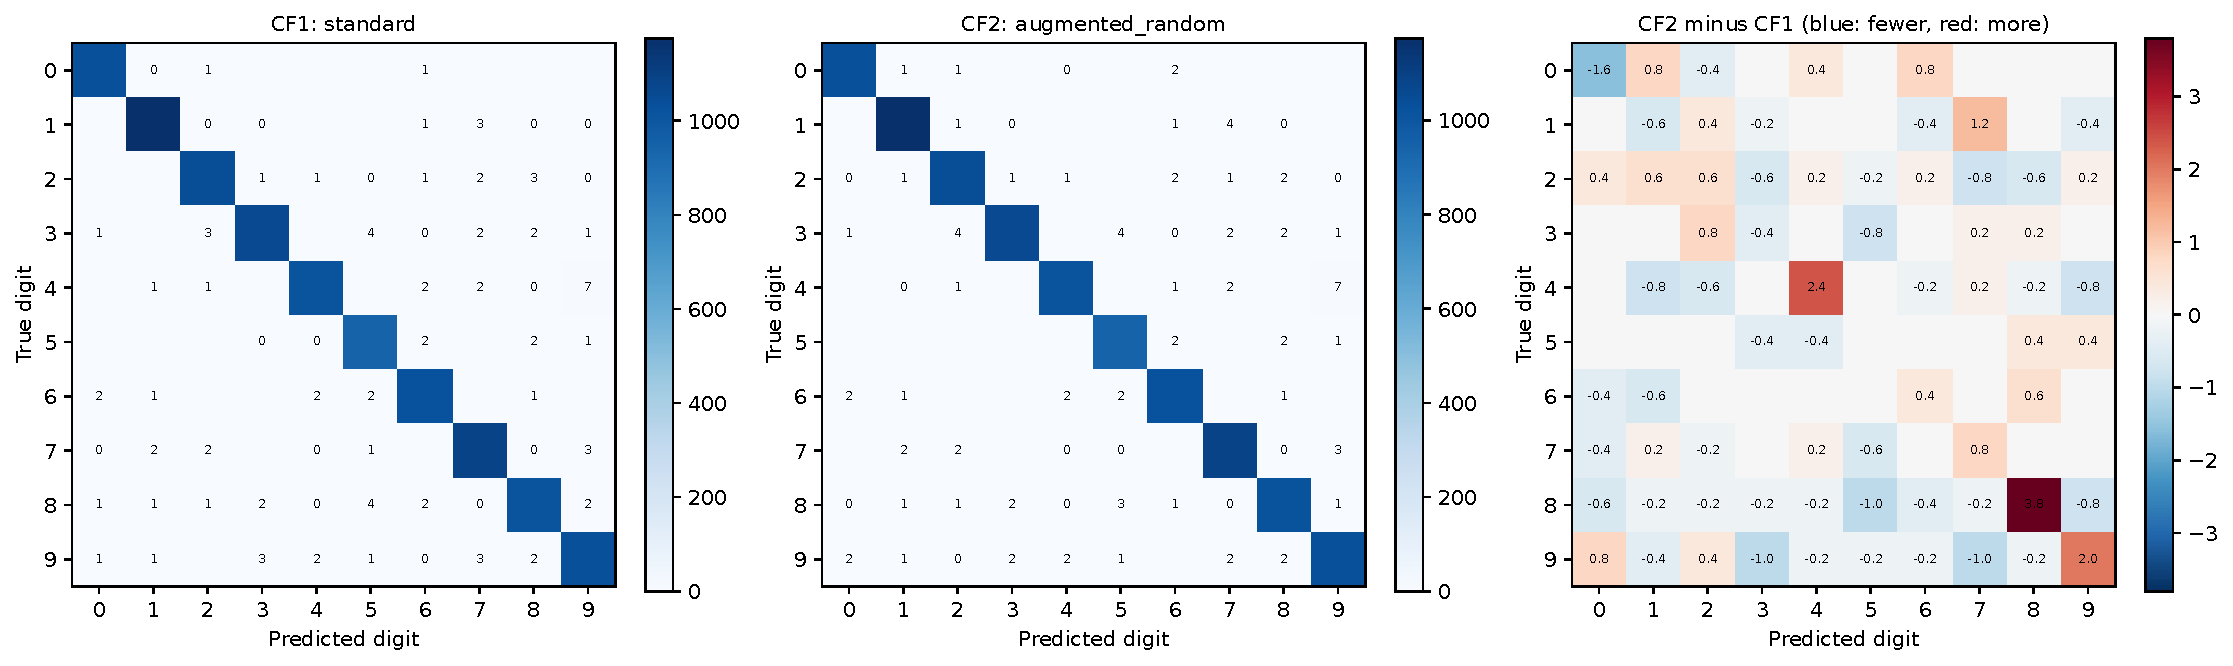
\includegraphics[width=\textwidth]{fig/targeted_augmentation/augmentation_comparison/confusion_standard_vs_augmented_random.pdf}\\[4pt]
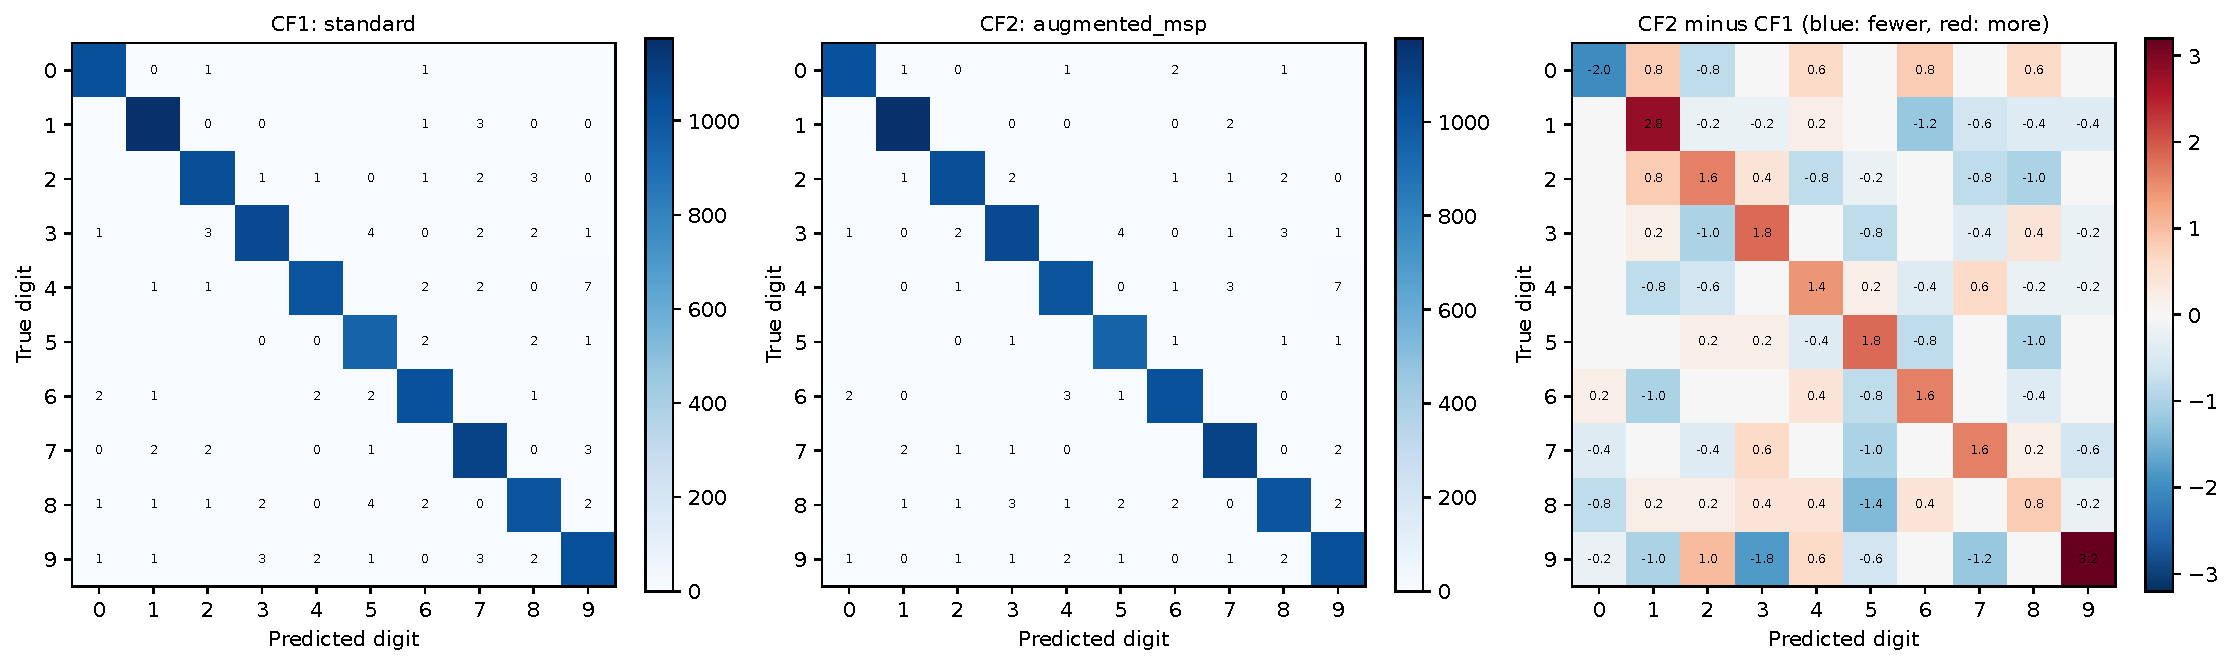
\includegraphics[width=\textwidth]{fig/targeted_augmentation/augmentation_comparison/confusion_standard_vs_augmented_msp.pdf}\\[4pt]
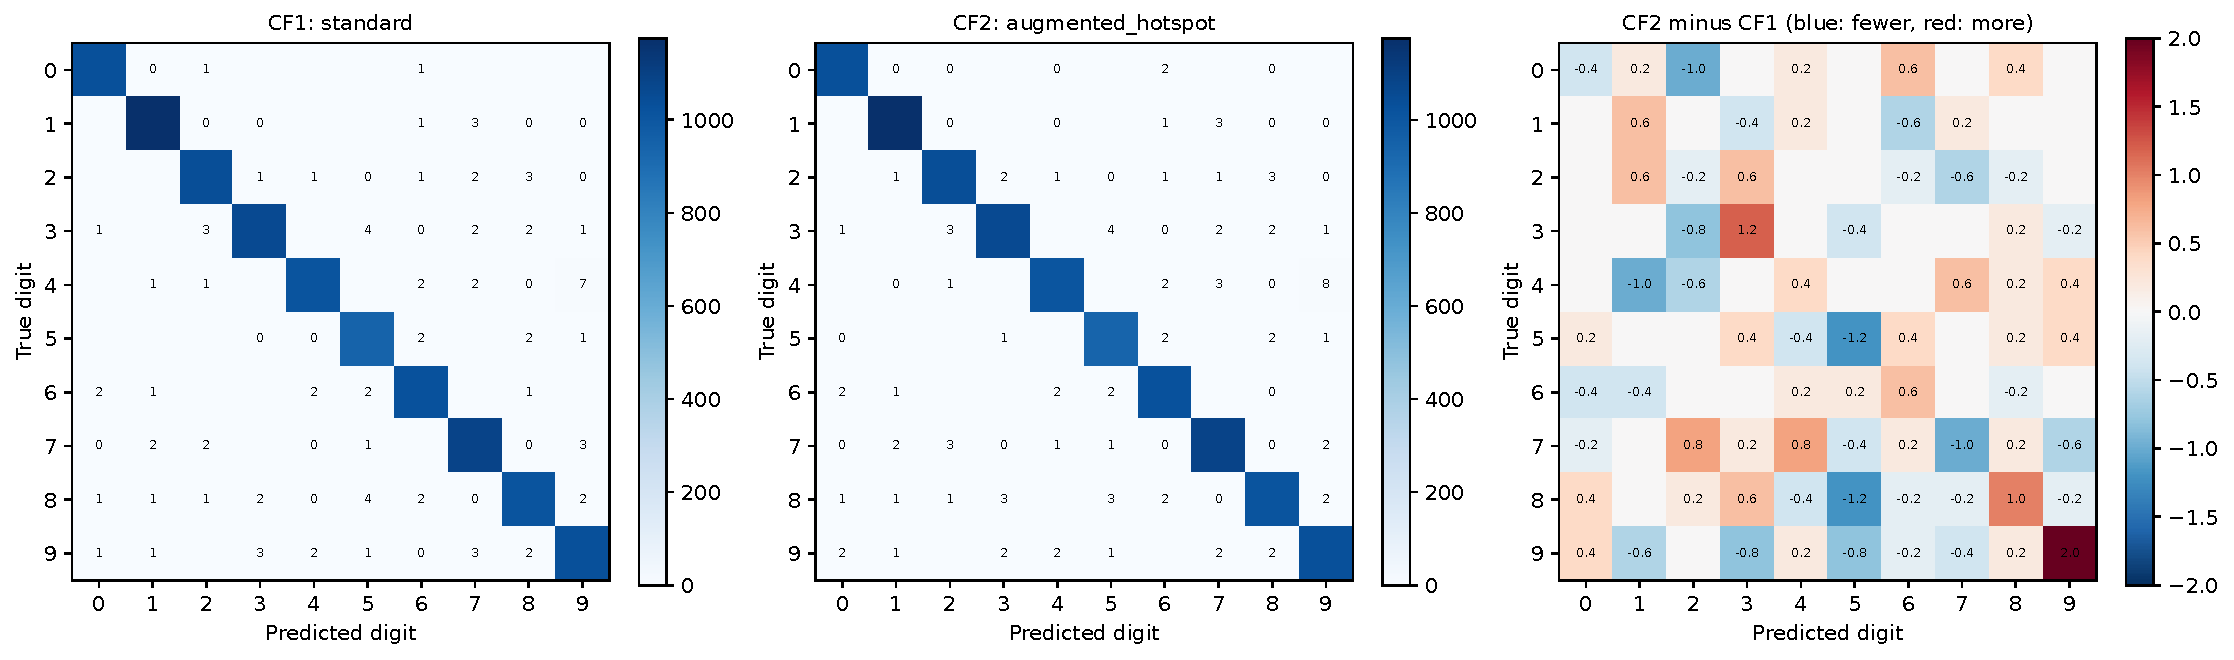
\includegraphics[width=\textwidth]{fig/targeted_augmentation/augmentation_comparison/confusion_standard_vs_augmented_hotspot.pdf}\\[4pt]
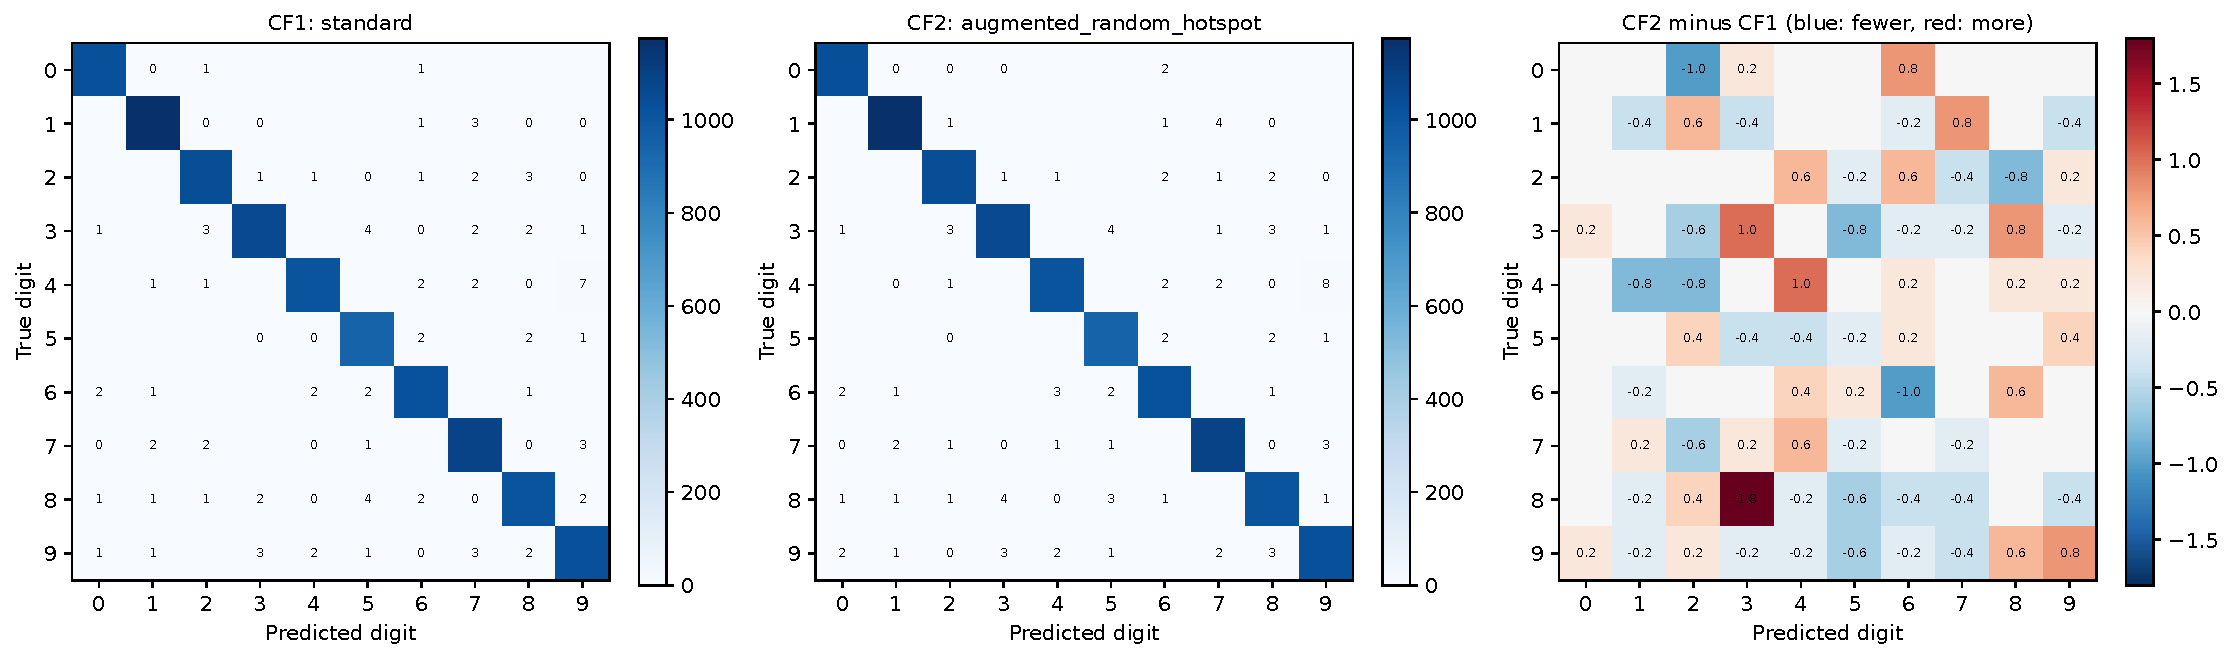
\includegraphics[width=\textwidth]{fig/targeted_augmentation/augmentation_comparison/confusion_standard_vs_augmented_random_hotspot.pdf}
\caption{CF2 of augmented\_random, augmented\_msp, augmented\_hotspot and augmented\_random\_hotspot (top to bottom).}
\end{figure}

\begin{figure}[H]
\centering
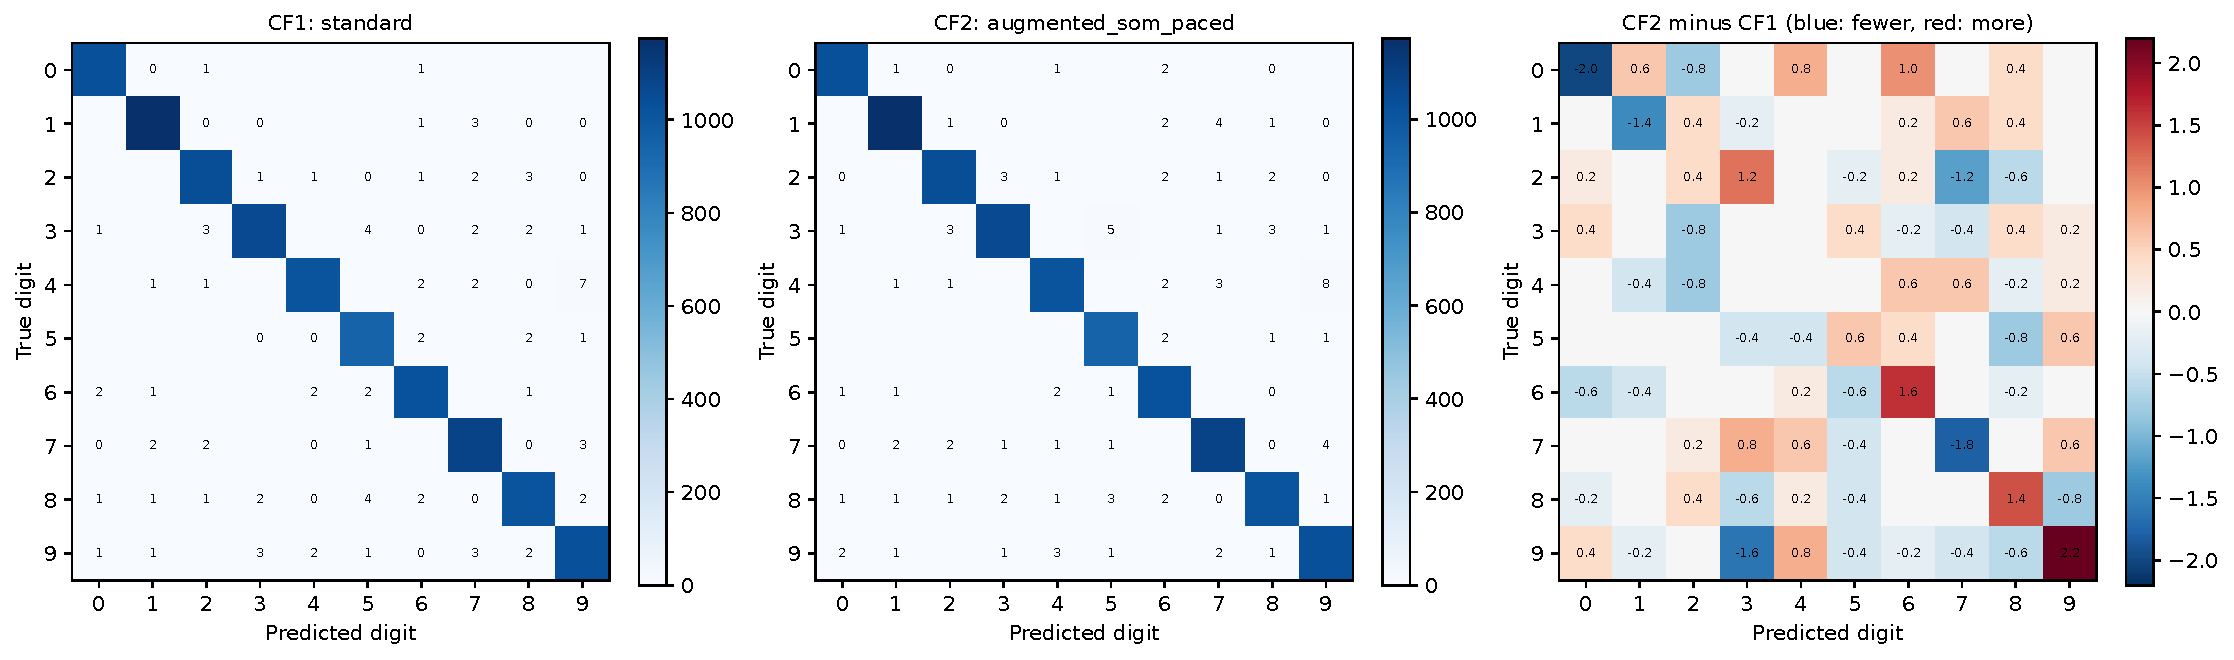
\includegraphics[width=\textwidth]{fig/targeted_augmentation/augmentation_comparison/confusion_standard_vs_augmented_som_paced.pdf}\\[4pt]
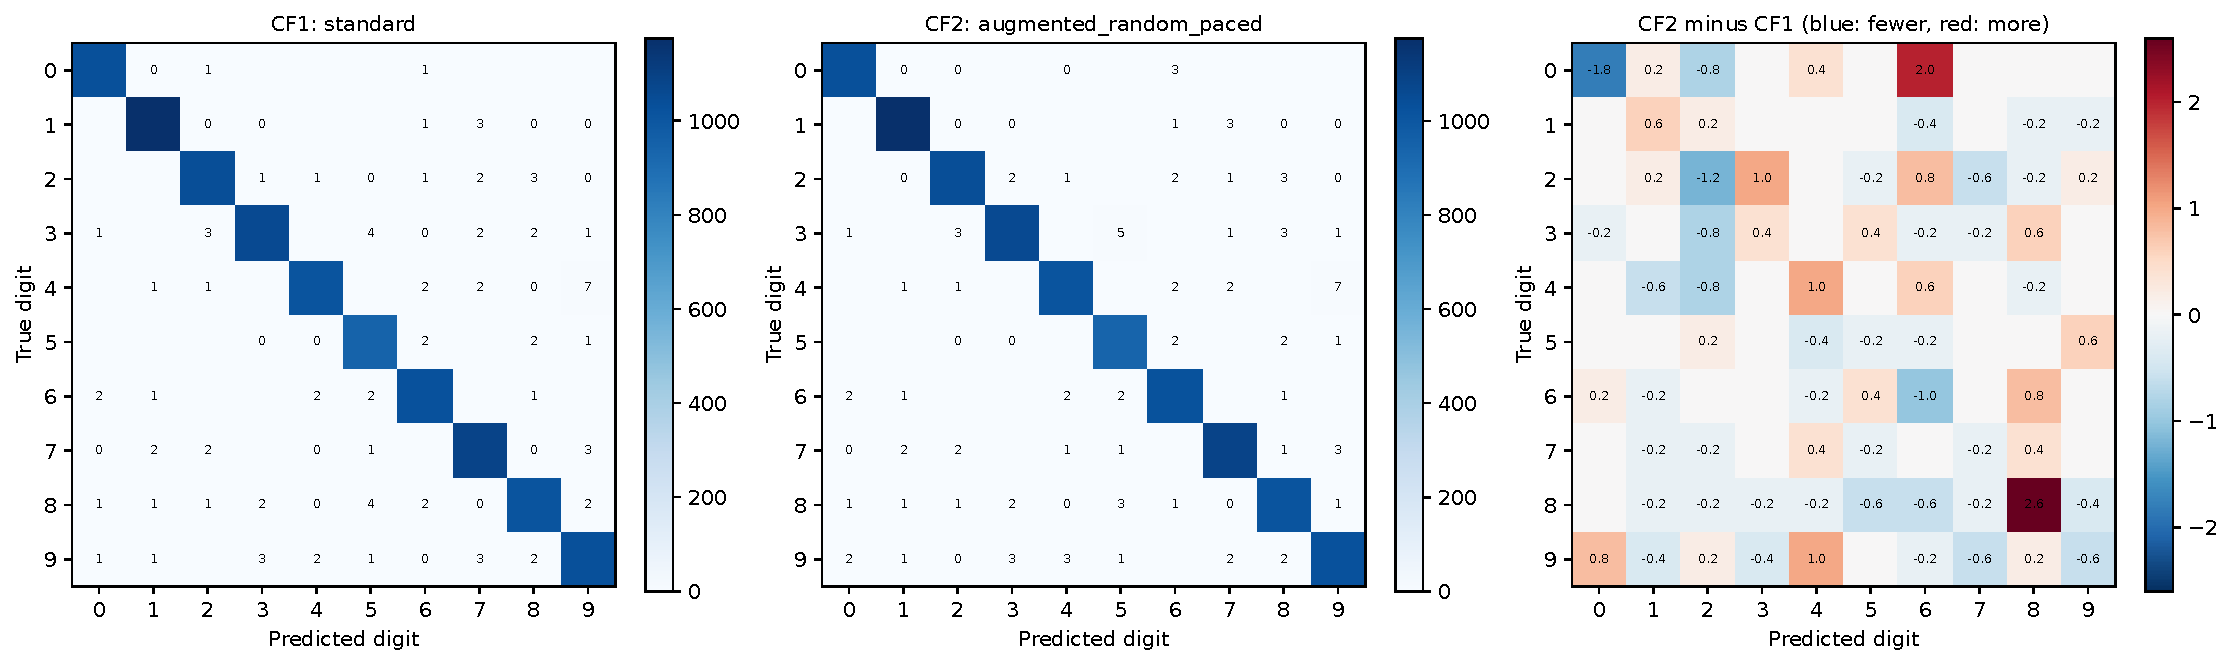
\includegraphics[width=\textwidth]{fig/targeted_augmentation/augmentation_comparison/confusion_standard_vs_augmented_random_paced.pdf}\\[4pt]
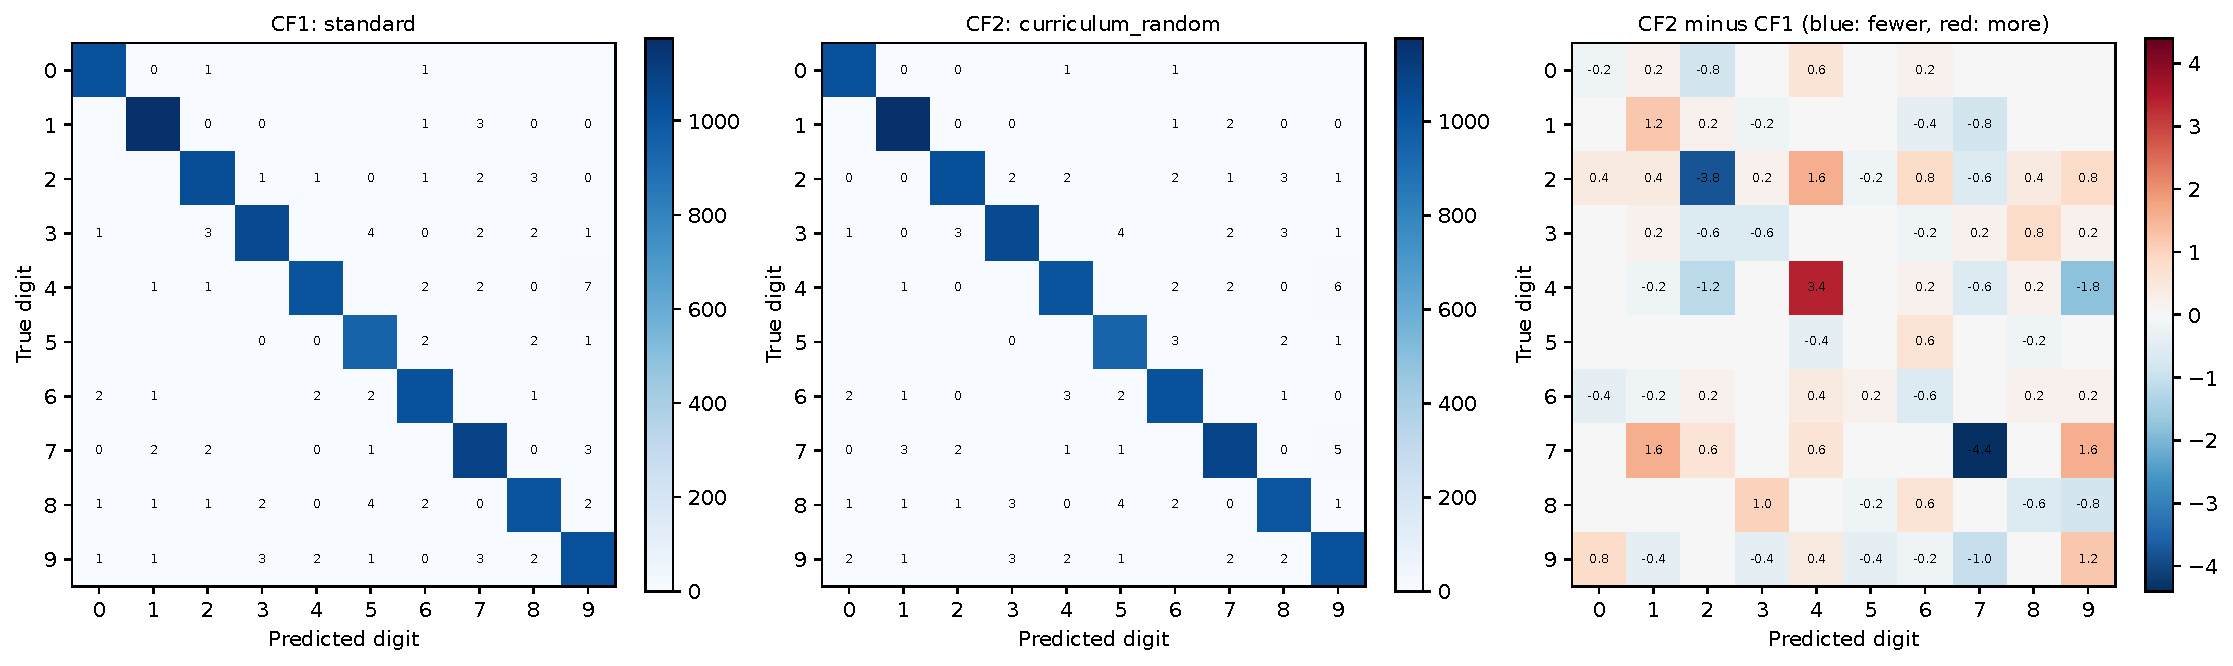
\includegraphics[width=\textwidth]{fig/hard_example_mining/curriculum_comparison/confusion_standard_vs_curriculum_random.pdf}\\[4pt]
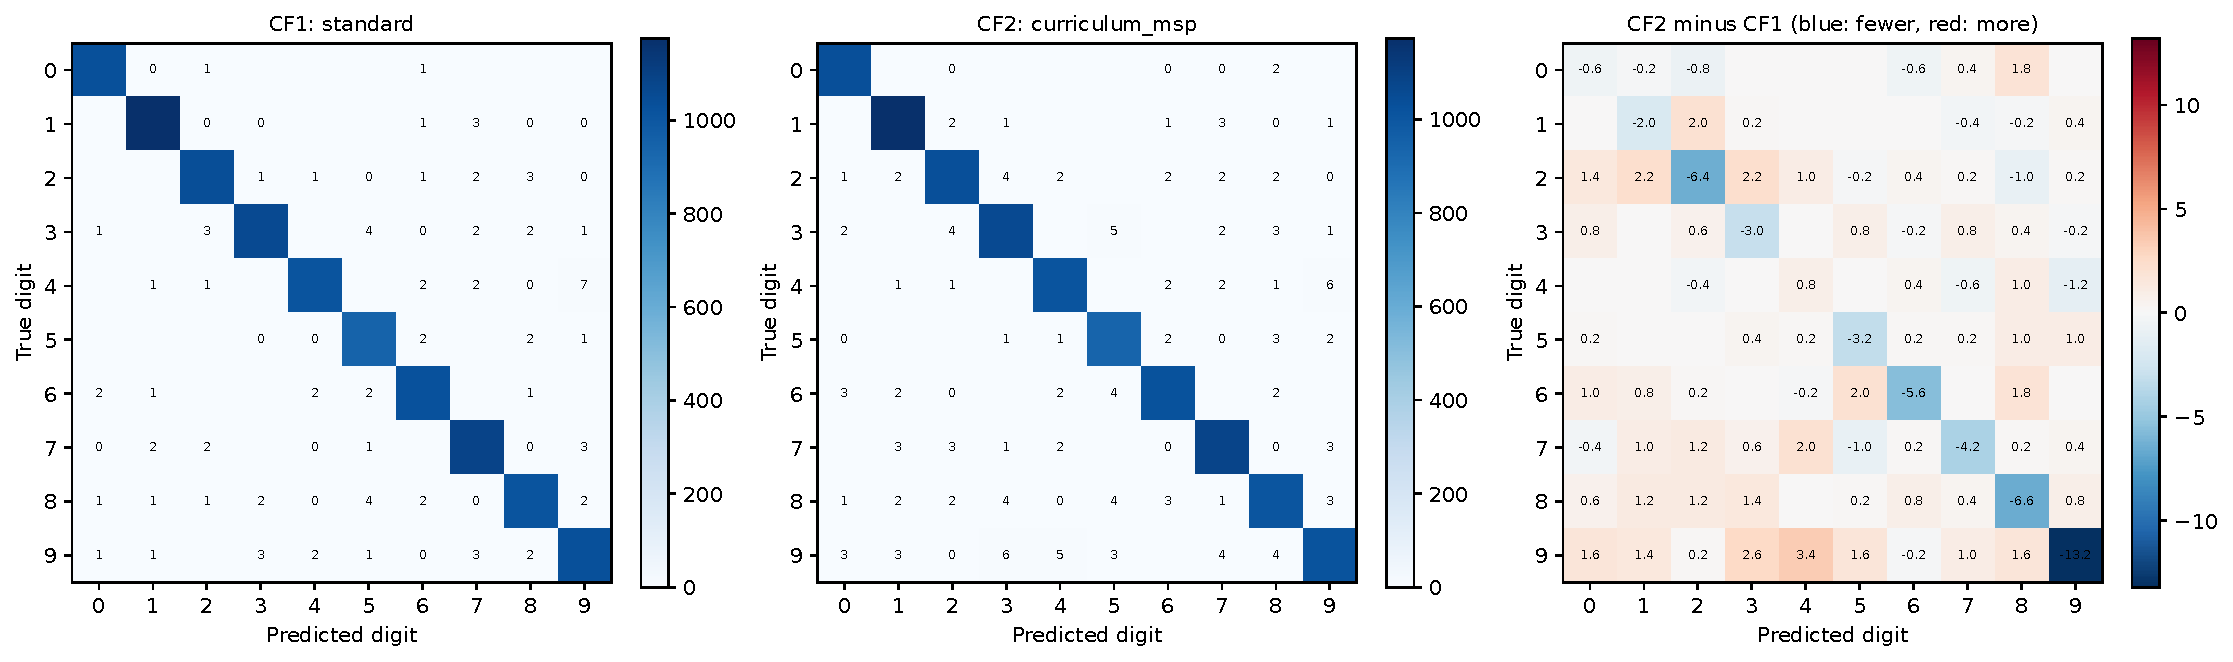
\includegraphics[width=\textwidth]{fig/hard_example_mining/curriculum_comparison/confusion_standard_vs_curriculum_msp.pdf}
\caption{CF2 of augmented\_som\_paced, augmented\_random\_paced, curriculum\_random and curriculum\_msp (top to bottom).}
\end{figure}

\begin{figure}[H]
\centering
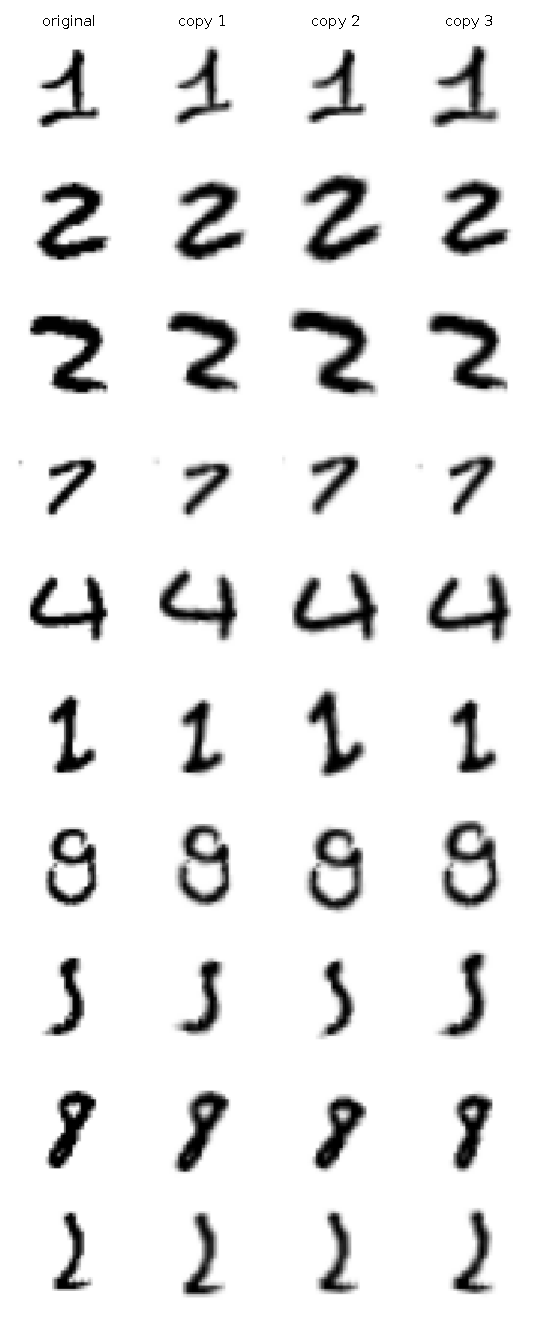
\includegraphics[height=0.55\textheight,keepaspectratio]{fig/targeted_augmentation/augmentation_comparison/augmentation_contact_sheet.pdf}
\caption{Ten training images from the hard pool (left column) and their three altered copies (shift up to 1 pixel, revision r2).}
\end{figure}

\begin{figure}[H]
\centering
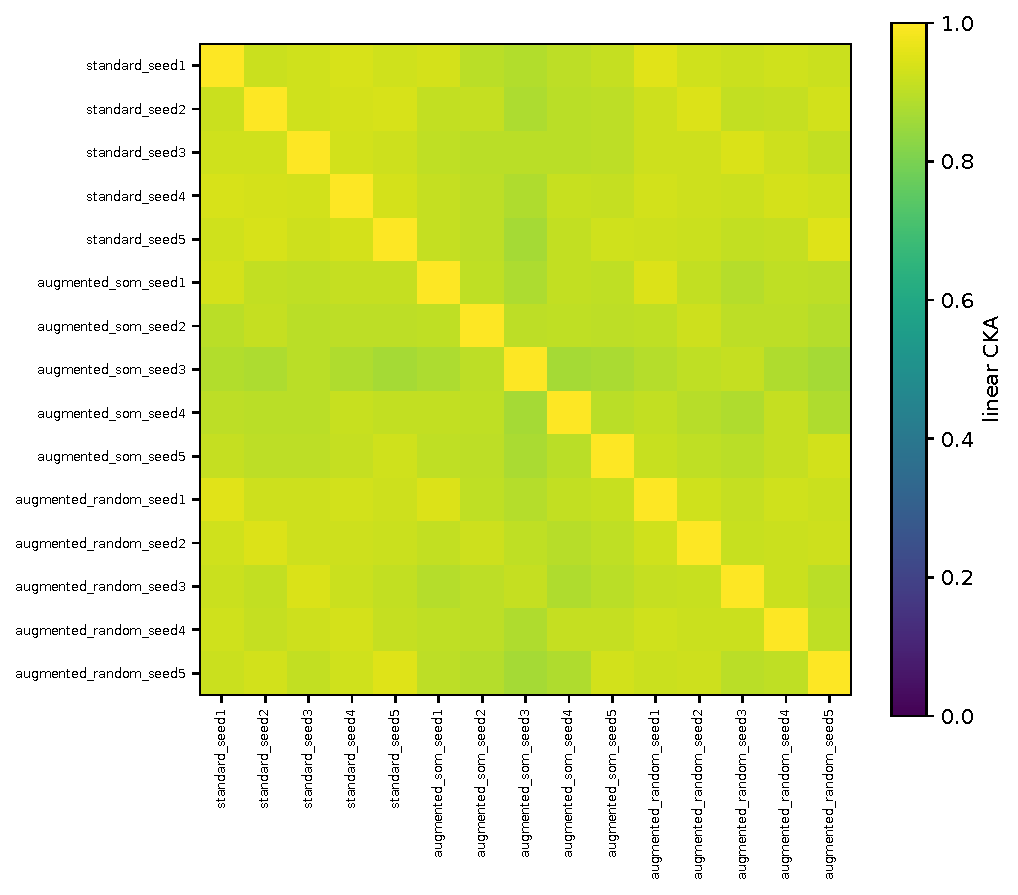
\includegraphics[width=\textwidth]{fig/som_reanalysis/embedding_similarity_cka.pdf}
\caption{Linear CKA between the embeddings of the 15 retrained networks (validation images).}
\end{figure}

\begin{figure}[H]
\centering
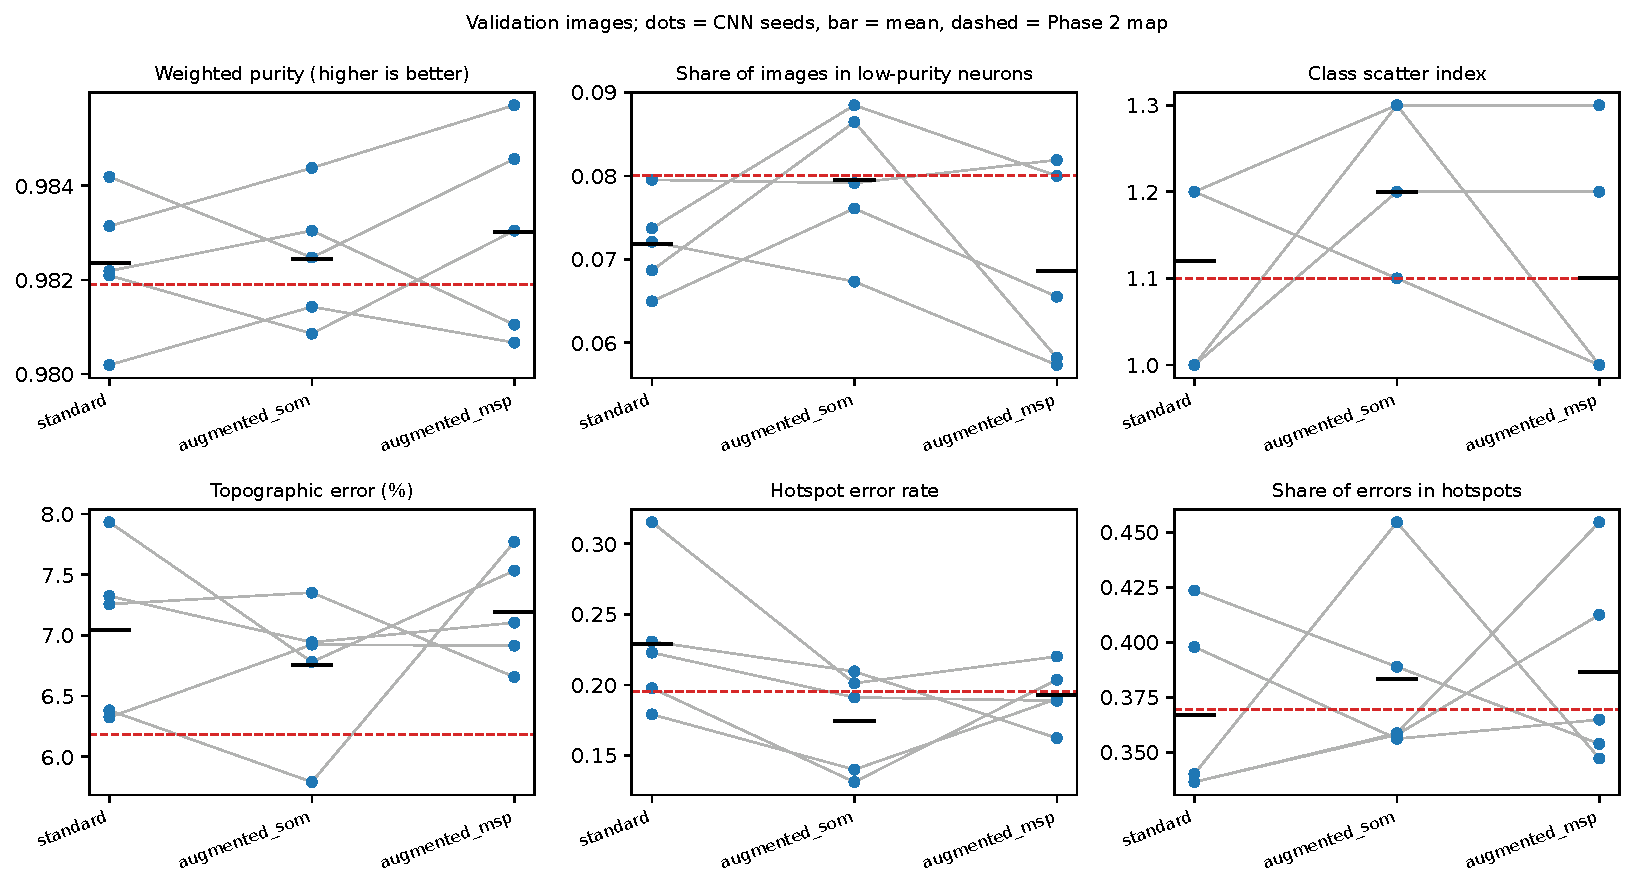
\includegraphics[width=\textwidth]{fig/som_reanalysis/msp_arm/map_measures_by_arm.pdf}\\[4pt]
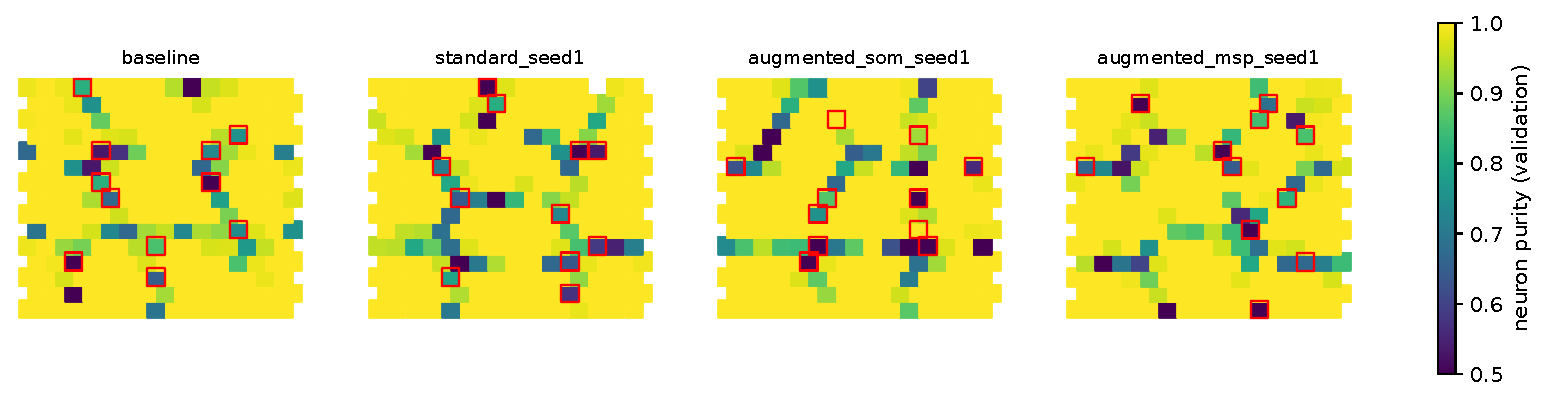
\includegraphics[width=\textwidth]{fig/som_reanalysis/msp_arm/purity_maps.pdf}
\caption{Secondary re-analysis run with the least-confident arm: map measures per arm (top, as in Figure~\ref{fig:reanalysis_measures}) and neuron purity maps, seed 1 (bottom, as in Figure~\ref{fig:reanalysis_purity}). The least-confident arm's new maps look like those of the other augmented arms.}
\end{figure}

\begin{figure}[H]
\centering
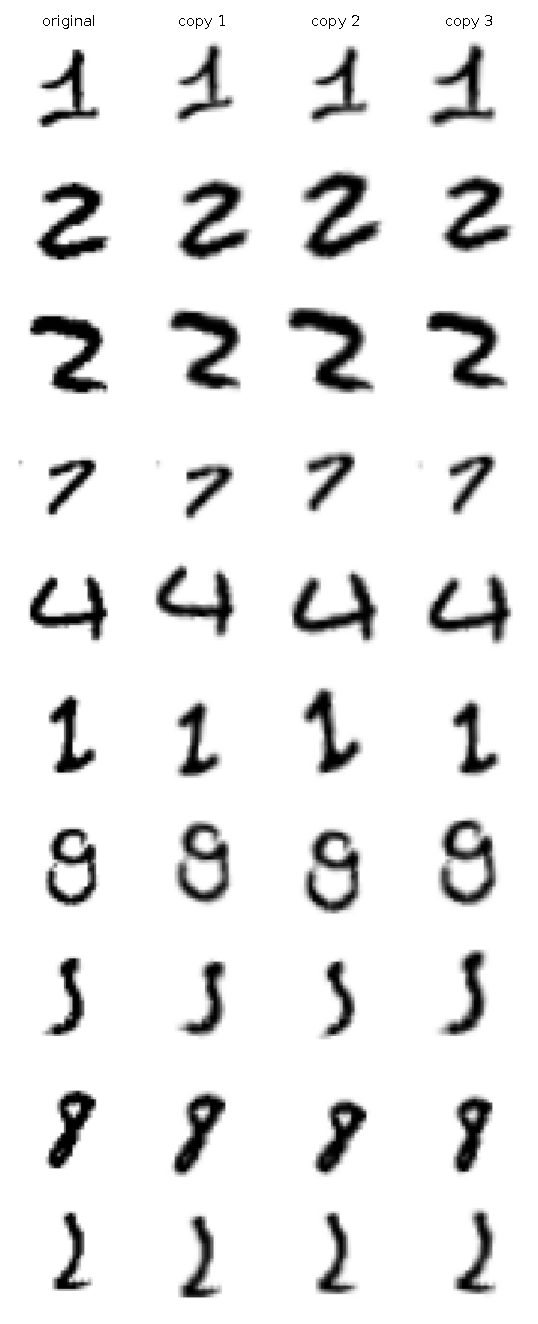
\includegraphics[height=0.5\textheight,keepaspectratio]{fig/targeted_augmentation/failed_check/augmentation_contact_sheet_r1.pdf}
\caption{The first augmentation ranges (shift up to 2 pixels, revision r1), which failed the transform check (validation accuracy 99.12\% to 95.83\%). Kept as the record; no arm was trained with them.}
\end{figure}

\end{document}
